%&pdflatex
\documentclass[11pt,a4paper]{scrreprt}

\usepackage[pdftex]{graphicx}

\usepackage{colortbl}	
\usepackage{xcolor}
\usepackage{soul}

\renewcommand{\familydefault}{\sfdefault}
\definecolor{uhhred}{cmyk}{0,100,100,0}
%!TEX encoding = UTF-8 Unicode
%!TEX root = hinweiseabschlussarbeit.tex

% Kodierung, Sprache, Patches {{{
\usepackage[T1]{fontenc}    % Ausgabekodierung; ermöglicht Akzente und Umlaute
                            %  sowie korrekte Silbentrennung.
%\usepackage[utf8]{inputenc} % Erlaubt die direkte Eingabe spezieller Zeichen;
                            %  utf8 muss die Eingabekodierung des Editors sein.
\usepackage[ngerman]{babel} % Deutsche Sprachanpassungen (z.B. Überschriften).
\usepackage{microtype}      % Optimale Randausrichtung und Skalierung.
\usepackage[
    autostyle,
    ]{csquotes}             % Korrekte Anführungszeichen in der Literaturliste.
%\usepackage{fixltx2e}      % Patches fuer LaTeX2e - seit 2015 nicht mehr nötig
\usepackage{scrhack}        % Verhindert Warnungen mit älteren Paketen.
\usepackage[
  newcommands
]{ragged2e}                 % Verbesserte \ragged...Befehle
\PassOptionsToPackage{
  hyphens
}{url}                      % Sorgt für URL-Umbrüche in Fußzeilen u. Literatur
% }}}

% Schriftarten {{{
\usepackage{mathptmx}       % Times; modifies the default serif and math fonts
\usepackage[scaled=.92]{helvet}% modifies the sans serif font
\usepackage{courier}        % modifies the monospace font
% }}}

% Biblatex {{{
\usepackage[
    style=alphabetic,
    backend=biber,
    %backref=true
    ]{biblatex}             % Biblatex mit alphabetischem Style und biber.
\bibliography{\jobname.bib} % Dateiname der bib-Datei.
\DeclareFieldFormat*{title}{
    \mkbibemph{#1}}         % Make titles italics
% }}}

% Dokument- und Texteinstellungen {{{
\usepackage[
    a4paper,
    margin=2.54cm,
    marginparwidth=2.0cm,
    footskip=1.0cm
    ]{geometry}             % Ersetzt 'a4wide'.
\clubpenalty=10000          % Keine Einzelzeile am Beginn eines Absatzes
                            %  (Schusterjungen).
\widowpenalty=10000         % Keine Einzelzeile am Ende eines Absatzes
\displaywidowpenalty=10000  %  (Hurenkinder).
\usepackage{floatrow}       % Zentriert alle Floats
\usepackage{ifdraft}        % Ermöglicht \ifoptionfinal{true}{false}
\pagestyle{plain}           % keine Kopfzeilen
% \sloppy                    % großzügige Formatierungsweise
\deffootnote{1em}{1em}{
  \thefootnotemark.\ }      % Verbessert Layout mehrzeiliger Fußnoten
\ifdefined\chapterformat
	\renewcommand*{\chapterformat}{% Hübscht Kapitelüberschrift mit senkrechtem 
		\thechapter\enskip%          grauen Balken zwischen Nummer und Text auf
		\textcolor{gray!50}{\rule[-\dp\strutbox]{2pt}{\baselineskip}}\enskip
	}
\fi
%\setkomafont{disposition}{\normalcolor\bfseries} % Aus der KOMA-Skript-Anleitung: „Mit dieser Änderung verzichten Sie darauf, für alle Gliederungsebenen serifenlose Schrift voreinzustellen“

\makeatletter
\AtBeginDocument{%
    \hypersetup{%
        pdftitle = {\@title},
        pdfauthor  = \@author,
    }
}
\makeatother
% }}}

% Weitere Pakete {{{
\usepackage{graphicx}       % Einfügen von Graphiken.
\usepackage{tabu}           % Einfügen von Tabellen.
\usepackage{multirow}       % Tabellenzeilen zusammenfassen.
\usepackage{multicol}       % Tabellenspalten zusammenfassen.
\usepackage{booktabs}       % Schönere Tabellen (\toprule\midrule\bottomrule).
\usepackage[nocut]{thmbox}  % Theorembox bspw. für Angreifermodell.
\usepackage{amsmath}        % Erweiterte Handhabung mathematischer Formeln.
\usepackage{amssymb}        % Erweiterte mathematische Symbole.
\usepackage{rotating}
\usepackage[
    printonlyused
    ]{acronym}              % Abkürzungsverzeichnis
\usepackage[
    colorinlistoftodos,
    textsize=tiny,          % Notizen und TODOs - mit der todonotes.sty von
    \ifoptionfinal{disable}{}%  Benjamin Kellermann ist das Package "changebar"
    ]{todonotes}            %  bereits integriert.
\usepackage[
    breaklinks,
    hidelinks,
    pdfdisplaydoctitle,
    pdfpagemode = {UseOutlines},
    pdfpagelabels,
    ]{hyperref}             % Sprungmarken im PDF. Lädt das URL-Paket.
    \urlstyle{rm}           % Entfernt die Formattierung von URLs.
%\usepackage{breakurl}
%\def\UrlBreaks{\do\/\do-}
\usepackage{listings}       % Spezielle Umgebung für Quelltextformatierung.
    \lstset{                
        language=C,
        breaklines=true,
        breakatwhitespace=true,
        frame=l,            % Linie links: l, doppelt: L
		framerule=2.5pt,    % Dicke der Linie
		rulecolor=\color{gray},% Farbe der Linie
        captionpos=b,
        xleftmargin=6ex,
        tabsize=4,
        numbers=left,
        numberstyle=\ttfamily\footnotesize,
        basicstyle=\ttfamily\footnotesize,
        keywordstyle=\bfseries\color{green!50!black},
        commentstyle=\itshape\color{magenta!90!black},
        identifierstyle=\ttfamily,
        stringstyle=\color{orange!90!black},
        showstringspaces=false,
        }
%\usepackage{filecontents}  % Direktes Einfügen von Dateiinhalt. Wird hier für
                            %  die Verwendung einer .bib-Datei in dieser .tex-
                            %  Datei benötigt.
% }}}
% \usepackage{parskip}
\addbibresource{main.bib}

\begin{document}

\title{Privatsphärewahrendes Anreiz- und Betrugserkennungssystem im Datentreuhandmodell}
\author{Knut Hoffmeister}

\newgeometry{centering,left=2cm,right=2cm,top=2cm,bottom=2cm}
\begin{titlepage}

\includegraphics[width=6.8cm]{up-uhh-logo-u-2010-u-farbe-u-rgb.pdf}
\begin{center}
    \vfill
    \Large Bachelorarbeit
    \vfill
    \makeatletter
    {\Large\textsf{\textbf{\@title}}}
    \makeatother
    \vfill
    vorgelegt von
    \par\bigskip
    \makeatletter
    {\@author}
    \makeatother
    \par
    Matrikelnummer 7509085 \par
    Studiengang Software System Entwicklung
    \vfill
    MIN-Fakultät \par
    Fachbereich Informatik
    \vfill
    \makeatletter
    eingereicht am {\@date}
    \makeatother
    \vfill
    Betreuer: Kevin Röbert
\end{center}
\ifoptionfinal{}{
    \begin{tikzpicture}[remember picture, overlay]
        \node[draw, red, font=\ttfamily\bfseries\Large, xshift=30mm, yshift=238mm, rotate=340, text centered, text width=6cm, very thick, rounded corners=4mm] at (current page.south) {Entwurf vom \today};
    \end{tikzpicture}
}
\end{titlepage}

\restoregeometry

\tableofcontents


\chapter*{Abstract}


%==================================================================================================


\chapter{Einleitung}
%``Die Bedeutung der Datenökonomie für die Entwicklung der Wirtschaftsleistung in Deutschland und Europa ist unbestritten`` \cite{falck2020rohstoff}\\
In der heutigen Zeit wird der fachgerechte Umgang mit Daten jeglicher Form, zunehmend wichtiger. Viele der großen Player wie Facebook oder Google, machen ihr Hauptgeschäft mit dem Verwenden von Nutzerdaten zu gewerblichen Zwecken, wie bspw. targeted Ads \cite{facebookad} \cite{googlead}. Und obwohl das Misstrauen eines Nutzers, solch eines großes Unternehmens gegenüber berechtigt ist, benötigen diese die gesammelten Daten auch, um neue Technologien zu entwickeln. Jedoch hat der Nutzer, der diese Daten generiert, meist keine Einsicht darüber, wer seine Daten verwendet und wofür diese zum Einsatz kommen. Ein potentieller Lösungsansatz für dieses Problem, ist die Verwendung von Datentreuhändersystemen. In einem Datentreuhändersystem, kann ein Endnutzer der Daten generiert zum einen seine Daten verschlüsselt bei einem Treuhänder lagert. Zum anderen ist der Treuhänder ein Mediator zwischen dem Endnutzer und einem Unternehmen, welches an den Daten interessiert ist. Möchte nun ein Unternehmen die Daten für ihre Zwecke verwendet, so kann dieses bei dem Treuhänder Daten anfordern. Daraufhin kontaktiert der Treuhänder den Nutzer, von dem die Daten stammen und fragt diesen, nach seiner Zustimmung. So kann der Nutzer genau einsehen, wer seine Daten verwenden möchte und kann unerwünschte Benutzung unterbinden. Das Ziel liegt hierbei vor allem darauf den Nutzer und seine Privatsphäre so gut wie möglich zu schützen.

In dieser Arbeit sollen, um die Motivation zur Benutzung eines Datentreuhänder zu erhöhen, zwei Forschungsfragen beantwortet werden: Wie kann ein privatsphäreschützender Anreiz zur Benutzung eines Datentreuhändermodells geschaffen werden? Und: Wie kann dieser Anreiz gegen Missbrauch geschützt werden? Aktuell ist der einzige Anreiz zur Benutzung eines Datentreuhändermodells für den Nutzer, der Schutz der Privatsphäre durch die Kommunikation über den Treuhänder. Um einen weiteren Anreiz zu bieten, soll hier ein Ansatz vorgestellt werden, welcher den Datengebenden für seine zur Verfügung gestellten Daten, angemessen entlohnt. Dies geschieht durch eine Transaktion von dem Datennutzenden an den Datengebenden, die trotz des Austausches von Zahlungsinformationen, die Privatsphäre des Datengebenden und dessen Identität so weit wie möglich schützt. Hierfür könnte bspw. eine leicht erweiterte Version des GNU Taler Zahlungssystem verwendet werden \ref{subsec:gnu}, um den Zahlungsverkehr zwischen den Parteien zu ermöglichen. Um dieses System vor Missbrauch zu schützen, wird ein Reputationssystem eingesetzt, um zu verhindern, dass ein Datengebender wertlose Daten oder qualitativ niedrig wertige Daten, in großer Masse bereitstellen kann, um so das System auszunutzen. Es soll zum einen, gleich wie der Bezahlvorgang, die Identität des Datengebenden schützen. Gleichzeitig soll es den Datennutzenden, der die Bewertung ausstellt, davon abhalten, das System durch mehrfaches Bewerten auszunutzen. Auch Betrugsversuche des Datengebenden sind nicht zu vernachlässigen, wie bspw. die Neuanmeldung eines Nutzers mit schlechter Reputation, um diesen Wert zurückzusetzen.

Dafür wird in dieser Arbeit der aktuelle Stand der Forschung in dem vorliegenden Kontext evaluiert und geprüft was bereits anwendbar und wo noch Lücken zur gewünschten Verwendung bestehen. Mit den gesammelten Forschungsergebnissen werden daraufhin mehrere Konzepte präsentiert, um das gerade genannte Ziel in das Treuhändermodell zu integrieren. Diese Konzepte werden des weiteren in ein bestehendes Treuhändersystem eingebaut, um konkrete Vergleichsgrundlagen zu erhalten. Bei dem hierfür vorgesehenen System, handelt es sich um das Tresor-Projekt der Universität Hamburg \cite{TRESOR}.


%==================================================================================================


\chapter{Hintergrund}
%\textit{Ausführlich erklären was das Problem mit konventioneller Datenkommunikation ist. Datentreuhänder einführen. Zeigen das Datentreuhänder das Problem lösen. Probleme mit Datentreuhänder ansprechen -> kein Anreiz zur Benutzung. Deswegen diese Arbeit als Anreiz und Betrugserkennung.}\\\\
Die zunehmende Digitalisierung unseres Alltags ist unabstreitbar \cite{dt-digitalisierung-stat}. Viele der täglichen Aktivitäten hängen stark mit ihr zusammen. Sei es den schnellsten Weg zu Arbeit finden mit Google Maps, das kontaktlose Bezahlen an der Kasse mit GooglePay oder Applepay, die Benutzung von Social Media zur Unterhalten oder der Onlinehandel über Anbieter wie Amazon. Sie alle liefern Komfort der durch die zunehmende Verwendung von Computern ermöglicht wird, welche im Hintergrund Unmengen an Daten für ihre Berechnungen verwenden. Diese Daten stammen meist von den Benutzern selbst. Bspw. die Standortdaten für die Berechnung potentieller Staus im Straßennetz \cite{dt-googlemaps-staus} oder die Unterhaltungsinteressen basierend auf Watchtime von bestimmten Social Media Inhalten. \\
Aufgrund des ständig wachsenden Markts für neue Digitaltechnologien ist auch die Nachfrage nach Daten über die letzten Jahr in Höhe gestiegen. Über das letzte Jahrzehnt haben Daten, Öl als wertvollste Ressource abgelöst \cite{dt-falck2020rohstoff}. Während 2008 die vier weltweit wertvollsten Unternehmen Ölkonzerne waren, waren 2018 bereits die 7 wertvollsten Unternehmen Internet- und Technologiefirmen. 

\section{Herkömmliche Datenkommunikation}
Unter anbetracht des hohen Wertes von Daten sind viele Unternehmen verständlicherweise sehr zurückhaltend was den Austausch betrifft. Schließlich beutet eine eigene Sammlung von Daten ein potentielles Verkaufsgut. Laut einer durch die Bundesregierung aufgegriffenen Studie von Fedkenhauer et al. geben zwar viele der befragten Unternehmen an, Aktivitäten im Bereich des Datenaustausches zu betreiben, allerdings umfasst das in 83\% der Fällen den Austausch von Daten mit Kundinnen und Kunden. 53\% der Unternehmen teilen ihre Daten mit Lieferantinnen und Lieferanten. Ein noch kleinerer Anteil von 21\% teilen ihre Daten mit Unternehmen aus der gleichen oder anderen Branchen und nur 15\% teilen sie mit Wettbewerbern \cite{dt-bundesregierung2021datenstrategie}. \\\\
Aus der kapitalgetriebenen Sicht eines Unternehmens besitzt das Teilen der eigenen Daten keinen direkten Nutzen. Da ein Unternehmen seine eigenen Gewinnmaximierung anstrebt, ist das Teilen von Daten eher ein Nachteil, da fremde Unternehmen mit den selbst gesammelten Daten ihre Produkte qualitativ erweitern können. Dadurch werden entweder andere Wettbewerben oder branchenfremde Unternehmen in ihrem Marktwert gefördert, was zu dem sinken des eigenen Marktwertes führt. \\
Diese protektive Herangehensweise kann allerdings auch der Gewinnmaximierung im Weg stehen. Im Fall von einem direkten Tausch an Daten können beide Parteien einen Profit aus der Interaktionen erwirtschaften. Die Bundesregierung selbst schreib in \cite{dt-bundesregierung2021datenstrategie} das kaum Datenkooperationen zwischen staatlichen und wirtschaftlichen Akteurinnen bestehen, obwohl die staatlich gesammelten Daten eine Grundlage für wirtschaftliche Innovation sein könnten. Im Gegenzug könnten die Daten von Unternehmen dem Staat bei der Sicherstellung seines Versorgungsauftrages, der Daseinsvororge und der Wahrung öffentlicher Schutzgüter helfen. Dies ist eine optimale Situation für die Verwendung eines Datentreuhänders.
\section{Datentreuhänder}
Ein Datentreuhänder ist ein neutraler vertrauenswürdiger Vermittler von Daten eines Datengebenden zu einem Datennutzenden. Er hat selbst kein kommerzielles Interesse an der Verwertung der Daten und agiert vergleichbar zu einem Notar strickt für den Datengeber. Seine Hauptaufgaben umfassen meist die Kontrolle von Zugriffsrechten, das Kontrollieren von Einhaltung der Datenschutzrichtlinien, sowie das verschlüsseln oder anonymisieren von Datenbeständen. In speziellen Fällen kann ein Datentreuhänder auch die Auswertung von Daten vornehmen. \cite{dt-bundesregierung2021datenstrategie}\cite{dt-richter2020ddvtalk}

Da wie bereits angeführt viele Unternehmen die Weiterleitung ihrer Daten vermeiden, ist unter der Annahme eines etablierten Datentreuhänders ein deutliche größerer Datenbestand verfügbar. Bereits heute - vor einer großen Etablierung von Datentreuhänder - verspricht das Konzept einige gesellschaftliche Vorteile: \cite{dt-richter2020ddvtalk}
\begin{enumerate}
    \item Durch sie können Datenbestände besser vernetzt werden und Zusammenhänge hergestellt werden, welche zu Innovationen führen.
    \item Der Wettbewerb unter Firmen wird gestärkt da mit besser zugänglichen Daten auch kleinere Unternehmen die kein Datenmonopol besitzen ihre Produkte aufwerten können.
    \item Der individuelle Endnutzer erhält mehr Kontrolle und Transparenz über die Speicherung und Verwendung seiner Daten.
\end{enumerate}

Allerdings ist das Verständnis eines Datentreuhänders nicht eindeutig. Jürgen Kühling beschreibt den Datentreuhänder als ``ein schillerndes Wesen. Jeder kennt ihn, jeder setzt ganz eigene Hofnungen in ihn – und jeder stellt sich doch etwas anderes unter ihm vor`` \cite{dt-kuhling2021datentreuhander}. Obwohl die Technologie eines Datentreuhänders bereits seit Jahren existiert und verwendet wird \cite{dt-hardinges2018data} ist es nicht gelungen eine konkrete allumfassende Definition für die Technologie zu finden.

%Ein Datentreuhänder ist ein neutraler vertrauenswürdiger Vermittler von Daten eines Datengebenden zu einem Datennutzenden. Dabei gilt zwischen dem Treuhänder und dem Datengebende eine sogenannte Treuhandschaft. Diese verpflichtet den Treuhänder die übermittelten Daten uneigennützig im Interesse des Datengebers zu verwalten. Die Aufgaben eines Datentreuhänders können die Qualitätsicherung der Datensätze, die Verwaltung von Zugangsrechten, die Einhaltung einheitlicher Standarts und Kontrollierung der Einhaltung von Datenschutzrechtlinien umfassen. \cite{bundesregierung2021datenstrategie}. 
%``Darüber hinaus gewährleisten sie eine Qualitätssicherung der Datensätze, verwalten Zugangsrechte und stellen die Einhaltung einheitlicher Standards sicher. Schließlich können Datentreuhänder auch im Interesse und zum Schutz von Verbraucherinnen und Verbrauchern tätig sein, auch im Bereich der personenbezogenen Daten``  \cite{bundesregierung2021datenstrategie}\\
\subsection{Definition}
 Die allgemeingültigste Definition stammt aus der Rechtswissenschaft und bezieht sich auf die Treuhandschaft im Allgemeinen. \textit{[Treuhandschaften sind ein] Rechtsverhältnis, bei dem eine natürliche oder juristische Person (Treugeber) einer zweiten Person (Treuhänder) ein Recht unter der Bedingung überträgt, von diesem Recht nicht zum eigenen Vorteil Gebrauch zu machen. [...] Gemeinsames Charakteristikum ist die Uneigennützigkeit und Vertrauenswürdigkeit bei der Wahrnehmung fremder Interessen bzw. die uneigennützige Ausübung von amtlichen Befugnissen"}\cite{dt-beeck2013treuhandschaft}. Diese Treuhandschaft wurde in der Vergangenheit verwendet, um bspw. Ländereien zu verwalten und im Namen einer lokalen Gemeinschaft Entscheidung zu treffen. \cite{dt-hardinges2018data}. In dem Fall eines Datentreuhänders bedeutet dies konkret, dass eine Datengebende Person beim bereitstellen ihrer Daten den Datentreuhänder dazu ermächtigt, über die Daten zu verfügen. Darunter fällt unter anderen auch die Weitergabe der Daten, solange die im Sinne des Datengebers ist. 

%``Data trusts are an approach to looking after and making decisions about data in a similar way that trusts have been used to look after and make decisions about other forms of asset in the past, such as land trusts that steward land on behalf of local communities. They involve one party authorising another to make decisions about data on their behalf, for the benefit of a wider group of stakeholders. With data trusts, the independent person, group or entity stewarding the data takes on a fiduciary duty. In law, a fiduciary duty is considered the highest level of obligation that one party can owe to another – a fiduciary duty in this context involves stewarding data with impartiality, prudence, transparency and undivided loyalty.``\cite{hardinges2018data}\\

%``For example, UK Biobank was set up in 2006 to steward genetic data and samples from 0.5m people and takes the form of a charitable company with trustees`` \cite{dt-hardinges2018data}\\

%``In Anlehnung an eine Bank, die für ihre Kundinnen und Kunden Vermögenswerte hält und verwaltet, verwalten Datentreuhänder gemäß dem engen Begriffsverständnis Daten für die Datengebenden in einem treuhänderischen Verhältnis. Als unabhängige dritte Partei validieren, kontrollieren und sichern sie Datenbestände der Datengebenden, teilen die Daten mit berechtigten Nutzenden im Sinne des Willens der Datengebenden und gewährleisten deren zweckgebundene Verwendung`` \cite{dt-lindner2021datentreuhänderschaft}\\

\subsection{Verschieden Modelle}
Insgesamt lassen sich alle bis zum heutigen Zeitpunkt in Betrieb genommenen oder geplanten Datentreuhandsysteme wie folgt kategorisieren. Zum einen besteht die Einteilung in Customer to Business oder Business to Business Systeme und zum anderen die risikobasierte Einteilung nach Zentralen/Dezentraler Datenspeicherung und Freiwilliger/Verpflichtender Nutzung. (siehe \ref{fig:dt-risikoeinteilug})

Die Unterscheidung zwischen Customer to Business und Business to Business Datentreuhändern basiert ausschließlich auf den interagierenden Parteien. Im Falle einer B2B Interaktion kommunizieren zwei Unternehmen die vorhandenen Daten miteinander. In diesem Fall kommt es häufig vor, dass eines der Unternehmen durch eine staatliche Behörde dargestellt wird. Bei den gespeicherten Daten handelt es sich meist um personenbezogene Daten. Aufgrund dessen befassen sich B2B Datentreuhänder häufig mit der Pseudonymisierung und der Verwaltung der bereitgestellten Daten. Sie sind unter anderem im Gesundheitswesen viel vertreten. \cite{dt-blankertz2020datentreuhandmodelle}
C2B Systeme umfassen solche, bei denen einen Endnutzer die Daten generiert  und diese an ein Unternehmen zur weiteren Benutzung freigibt. Ihre Aufgabe ist hauptsächlich die Unterstützung des Nutzers bei der gerechten Weiterverarbeitung seiner Daten. \cite{dt-blankertz2020datentreuhandmodelle} Hier sind dementsprechend die Pseudonymisierung der Daten sowie die Einhaltung von Datenschutzrechtlinien und einheitlicher Standarts die Hauptziele des Datentreuhänders.

Des weiteren lassen sich Datentreuhandsysteme anhand ihrer Datenspeicherung sowie Nutzung kategorisieren und Risikotechnisch bewerten. Die zentrale Speicherung der Daten bietet einige Vorteile für den Treuhänder. Sie ermöglicht es Daten vor zu verarbeiten, zu analysieren und Datenverarbeitende von dem direkten Zugang der Daten auszuschließen. Allerdings birgt die zentrale Datenspeicherung ein enormes Risiko der Datensicherheit, da hier ein single point of failure entsteht. Bei einem Angriff auf einen solchen Datentreuhänder fällt es einem Angreifer somit leichter eine große Menge an Daten zu stehlen.
Bei einer dezentralen Speicherung werden die Daten durch den Treuhänder pseudonymisiert oder ganz anonymisiert und bei dem Datengeber gelagert. Aus diesem Grund bietet eine dezentrale Datenspeicherung mehr Sicherheit vor Diebstahl. Sie zieht allerdings auch eine eingeschränkte Verarbeitung und Analyse der Daten mit sich und erhöht die Komplexität der Verwaltung.\\

Es besteht eine weitere Unterteilung in Datentreuhandsysteme, dessen Benutzung freiwillig ist oder verpflichtend ist. Dabei fällt der größte Anteil an Systeme unter die freiwillige Benutzung. Es gibt jedoch auf Szenarien in denen die Verwendung einer Datentreuhand verpflichtend ist. Ein Beispiel hierfür wäre das Krebs- und Transplantationsregister aus dem medizinischen Bereich. Das Risiko steigt bei verpflichtenden Systemen, da sie meist einen wichtigen Bestandteil der Kommunikation ausmachen der nicht umgangen werden kann. Somit sind die potentiellen Schäden die bei einem Angriff entstehen können höher als in einem freiwilligen System.

\begin{figure}
    \centering
    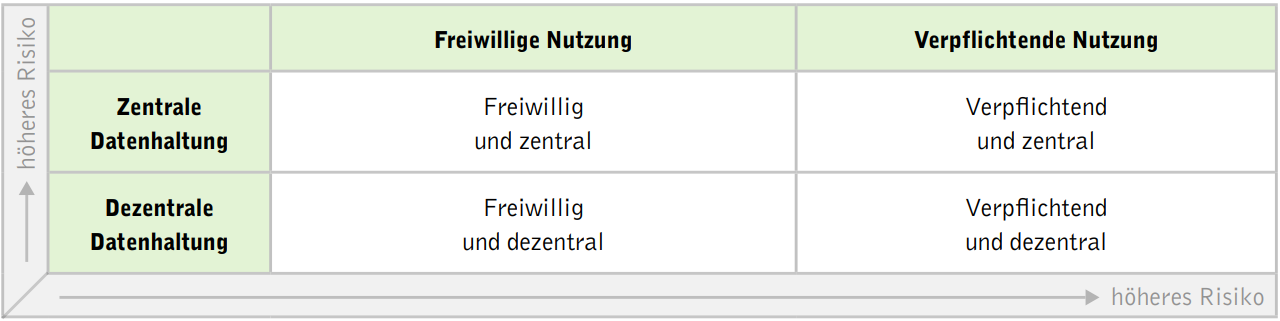
\includegraphics[width=0.9\textwidth]{DT-RisikoEinteilung.png}
    \caption{Risikobasierte Unterscheidung von Datentreuhandmodellen \cite{dt-blankertz2021neue}}
    \label{fig:dt-risikoeinteilug}
\end{figure}

\section{Anwendungsfälle}
\label{sec:dt-usecases}
Das mögliche Spektrum an Anwendungsfällen ist denkbar breit. In beinahe jedem Bereich der eine große Menge an Daten benötigt oder verwaltet ist die Verwendung eines Datentreuhänders angedacht. Beispiele dafür sind:
\begin{itemize}
    \item \textbf{Patientendaten} Der Datentreuhänder sorgt für eine pseudonymisierung von Patientendaten zur Bereitstellung an Forschungseinrichtungen. Hierbei behält der Patient die Hoheheit über seine Daten und kannst selbst entscheiden mit wem seine Daten geteilt werden.
    \item \textbf{Autonomes Fahren} Beim autonomen Fahren werden enorm viele Daten generiert, welche seit 2017 per Gesetz gespeichert werden müssen \cite{dt-bundesdruckereiDatentreuhänder}. Leider ist die Zugehörigkeit der Daten rechtlich weder dem Autohersteller noch dem Autoinhaber zuzuschreiben \cite{dt-richter2020ddvtalk}. An dieser Stelle kann ein Datentreuhänder die Kommunikation erleichtern und exklusiven Zugang von bspw. Versicherungen oder Automobilkonzernen ausschließen.
    \item \textbf{E-Government} Durch die Verwendung eines Datentreuhänders können bei der behördlichen Verwaltung von Bürgerdaten große Fortschritte erzielt werden. Unter anderem müssen so notwendige Informationen aus anderen Registern für Verwaltungsvorgänge nicht mehr vom Bürger bereitgestellt werden. Der Bürger gibt lediglich seine Einwilligung zum Abruf der Daten zu Beginn des Verwaltungsvorgangs. Auf diese Weise können Verwaltungsvorgänge erheblich effizienter Ablaufen.
    \item \textbf{KI-Datenpools} Eines der größten Probleme bei Entwicklung von KI-Software ist der Zugang zu einer ausreichend großen Menge an Trainingsdaten. Ein Datentreuhänder kann solche Daten die zur Verwendung für KI Training freigegeben wurden sammeln und pseudonymisiert an mehrere Interessierte verteilen. Dadurch entsteht ein einheitlicher Zugang zu Trainingsdaten der gleichzeitig nur freigegebene Daten beinhaltet und so rechtlichen Streit über das Copyright aus dem Weg geht.
    \item \textbf{Industrie} In der Industrie besteht eine hohe Abhängigkeit von Warenbewegungen, seien es in Lieferketten, Logistik oder Handel. Durch die Verwendung eines Datentreuhänders können diese Informationen pseudonymisiert an Warenempfänger weitergegeben werden. Vor allem in diesem Bereich besteht durch die Zusammentragung an Lieferinformationen in Kombination mit Algorithmen der Graphentheorie ein großes Innovationspotential.
    \item \textbf{PIMS} Personal Information Management Systeme befassen sich grundsätzlich mit der Wahrung von personenbezogenen Daten und bietet ihren Nutzern mehr Kontrolle über diese.  Datentreuhänder sind für solche Systeme vor allem von Vorteil da sie im Umgang mit personenbezogenen Daten dem Nutzer wieder die Kontrollen über seine Daten zurückgeben.
\end{itemize}
\cite{dt-blankertz2021regulierung}\cite{dt-blankertz2021neue}\cite{dt-bundesdruckereiDatentreuhänder}

Der erste Datentreuhänder entstand einer bereits im Jahre 2006 in England. Seit dem das Thema Datentreuhänder in den letzten Jahren immer mehr zum Trend wurde \cite{dt-richter2020ddvtalk}. Die ``UK Biobank`` ist eine biomedizinische Datenbank die sowohl medizinische Daten als auch biologische Proben von einer halben Millionen Teilnehmer aus Großbritanien speichert\cite{dt-hardinges2018data}. Die gespeicherten Daten sind pseudonymisiert und werden ausschließlich an Forscher im Feld der Medizin weitergegeben, was die UK Biobank zu einem Paradebeispiel für einen Patientendatentreuhänder macht.

% Zwar ist die Bereitschaft persönliche Daten über einen Datentreuhänder zu teilen größer als ohne einen Datentreuhänder wie \cite{dt-tresor24study} zeigt.


\section{Bestehende Anreize}
Generell sei gesagt, dass die Verwendung eines Datentreuhänders keine direkten Nachteile mit sich bringt. Wenn Daten ohnehin geteilt werden oder werden müssen, so behält der Nutzer bei der Speicherung der Daten über einen Datentreuhänder mehr Kontrolle über die Verwendung seiner geteilten Daten verglichen mit dem direkten Teilen mit Unternehmen. Durch den Datentreuhänder wird ihm ermöglicht zu einem beliebigen Zeitpunkt das weitere Teilen seiner Informationen einzustellen. Vermutlich teilen deswegen Privatpersonen ihre Daten lieber mit Datentreuhändern als auf direktem Weg. \cite{dt-tresor24study}

Allerdings gibt es nur wenige Vorteile die die freiwillige Benutzung eines Datentreuhänders reizvoll machen. Bei freiwilligen C2B Datentreuhändern, hängt die Entscheidung für oder gegen die Nutzung des Treuhänders beim Nutzer. Es ist also an ihm abzuwägen ob die Verwendung ausreichend Vorteile liefert. Im Fall von PIMS Treuhänder wird die Verwendung von manchen als erstrebenswert angesehen, da der Nutzer mehr Kontrolle über die Verbreitung von persönlichen Daten erhält und selbst entscheiden kann, mit wem diese geteilt werden. Die Erkenntnissen von Jai et al. \cite{dt-jai2016privacy} zeigen hingegen, dass vor allem jüngere Erwachsene weniger Wert auf den Schutz ihrer persönlichen Daten legen.

Allerdings gibt es keinen direkten Anreiz zur Verwendung einer solchen Software oder der Weitergabe der persönlichen Daten, da nur das Business von den gesammelten Daten einen Mehrwert hat. Der Nutzer der seine Daten freigibt erhält keine Kompensation in irgendeiner Form. Folglich kann es für einen Datentreuhänder dessen Verwendung freiwillig ist mühsam sein neue Nutzer zu gewinnen und die Technologie als solche auszubauen.


%==================================================================================================


\chapter{Anforderungen und verwandte Arbeiten}
\section{Anforderungen}
\label{sec:req}
Da eine Lösung zur Verwendung durch einen Datentreuhänder konzeptioniert ist, decken sich die Anforderungen an eine mögliche Lösung stark mit denen eines üblichen Datentreuhänders. Im Grunde kann zwischen funktionalen und nichtfunktionalen Anforderungen unterschieden werden.

\subsection{Funktionale Anforderungen}
\label{enum:req:funktional}
\begin{enumerate}
    \item Ein Bezahlsystem ermöglicht es einem Datengebenden Geld für seine Daten zu erhalten.
    
    \item Die Präsenz eines Reputationswertes gibt den Datennutzenden vor Erwerb der Daten eine Einschätzung über deren Qualität.
    \item Nach Abschluss der Transaktion kann ein Datennutzender den entsprechenden Datengebenden aufgrund der Qualität der übermittelten Daten bewerten.
    \item Ein Datengebender muss eine Bewertung seiner Daten ermöglichen.
    \item Ein Datennutzender kann pro Austausch nur genau eine Bewertung für einen Datengebenden abgeben. Mehrfache Bewertungen ist nur im Fall von mehrfachem Erwerb möglich.
\end{enumerate}

\subsection{Nicht funktionale Anforderungen}
\label{enum:req:nichtfunktional}
\begin{enumerate}
    \item \textbf{Anonymität} Die Identität des Datengebenden darf durch den Austausch von Zahlungsmitteln oder durch dessen Reputation nicht nachverfolgbar sein.
    \item \textbf{Zeitsensitivität} Der Bezahlvorgang muss in vernachlässigbarer Zeit geschehen.
    \item \textbf{Skalierbarkeit} Die Rechenzeit des Systems soll bei linear steigender Menge an Datengebenden und Datennutzenden auch mit linearem Zeitaufwand zunehmen.
    \item \textbf{Vertraulichkeit} Die kommunizierten Daten dürfen nicht durch unbefugte Dritte ausgelesen werden können.
    \item \textbf{Integrität} Die kommunizierten Daten dürfen nicht unbemerkt durch unbefugte Dritte verändert werden.
\end{enumerate}


\section{GNU Taler}
\label{subsec:gnu}
Das im Paper ``Enabling Secure Web Payments with GNU Taler`` von J. Burdges et al. eingeführte Zahlungssystem GNU Taler, ist ein elektronisches Online-Zahlungssystem, das Datenschutz für Customer und Mechanismen zur steuerlichen Nachverfolgung für Merchants bietet \cite{gnu-burdges2016enabling}. Es verwendet einen Exchangeservice, um Münzen mithilfe von blinden Signaturen zwischen Nutzern und Händlern zu transferieren. Im Folgenden werden diese Münzen als Taler bezeichnet, um Verwirrung zu vermeiden. Das System basiert auf 4 übergeordneten Rollen, dessen Interaktion grob in Abbildung \ref{fig:gnu_taler_overview} skizziert ist. Der Customer möchte ein Gut oder eine Dienstleistung bei dem Merchant erwerben und bezahlt diesen dafür mit Talern, welcher er beim Exchange erworben hat. Der Merchant kann die erhaltenen Taler wieder beim Exchange für herkömmliche Währungen eintauschen. Ein Auditor überprüft währenddessen die Liquidität des Exchange, um sicherzustellen, dass dieser auch bei Datenverlust von Taler noch in der Lage ist allen Beteiligten, Auszahlungen zu ermöglichen.

\begin{figure}[H]
    \centering
    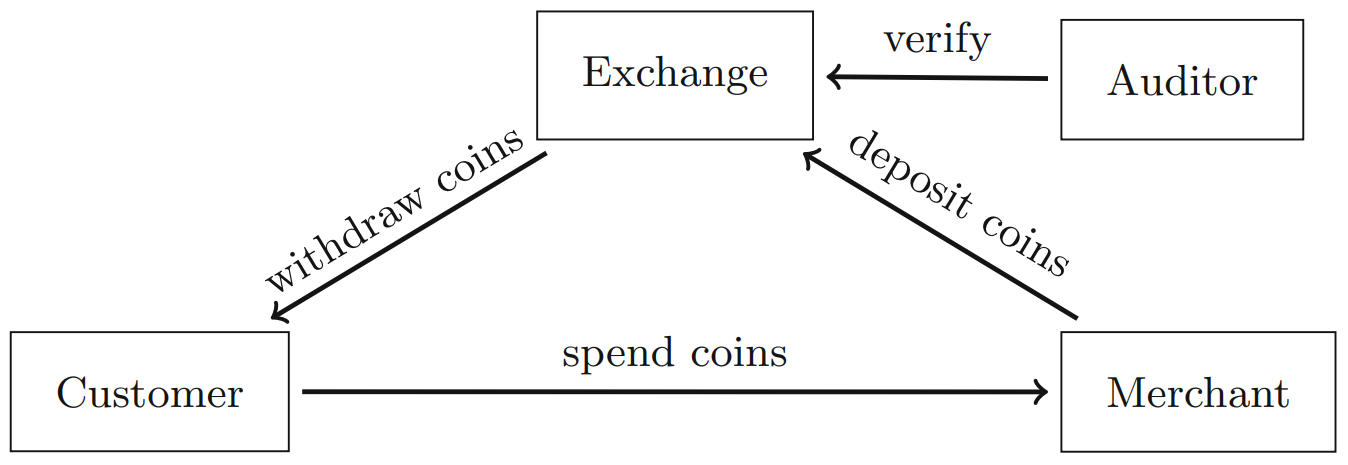
\includegraphics[width=0.7\textwidth]{gnu_system_graphic.png}
    \caption{Grundlegender Ablauf des GNU Taler Systems \cite{gnu-burdges2016enabling}}
    \label{fig:gnu_taler_overview}
\end{figure}

\textit{Taler abheben.} Damit ein Customer Geld auf sein Wallet laden kann, muss er sich zuerst bei seiner Bank anmelden. Sollte die Bank GNU Taler native unterstützen, so kann der Customer in einem Formular eine Summe auswählen, die er in Taler übertragen möchte und einen Exchangeservice, über welchen der Tausch abgewickelt wird. Nachdem der Customer die Transaktion bestätigt hat, wird die ausgewählte Summe transferiert, der Exchangeservice signiert die equivalente Summe an Talern und überträgt diese in das Wallet des Customers.

\textit{Taler ausgeben.} Gehen wir von der Situation aus, dass eine Customer bei einem Merchant (hier ein Onlineshop), etwas erwerben möchte. Nach der Auswahl des Produktes und GNU Taler als Zahlungsmittel, erstellt der Merchant einen Zahlungsvertrag, der Details wie den Gesamtpreis, mögliche offene Umwandlungsgebühren und akzeptierte Exchangeservices beinhaltet und sendet diesen an das Wallet des Customers.  Wenn der Customer daraufhin die Zahlung übermittelt, so leitet der Merchant die erhaltenen Taler direkt an den Exchange weiter. Wenn der Exchange den Eingang bestätigt, so kann der Merchant dem Customer die Transaktion bestätigen und der Kauf ist somit abgeschlossen. 


In dem Treuhändermodell eignet sich GNU Taler aber nur teilweise als Zahlungssystem. Der Datengebende stellt dabei den Merchant da, der seine Daten als digitales Gut anbietet. Der Datennutzende stellt hier die Rolle des Customers dar und möchte diese Daten erwerben. Sollte der Datengebende der Anfrage des Datennutzende zustimmen, so würde er einen Zahlungsvertrag formulieren, um den Anspruch auf seine Vergütung zu formalisieren. Allerdings soll der Datengebende im Datentreuhändermodell so gut wie möglich vor Informationsgewinnung geschützt werden. Bei dem von GNU Taler vorgeschlagenen Prozess wird jedoch die Identität des Datengebenden nachverfolgbar, während der Datennutzenden anonym bleibt. Zusätzlich besteht eine direkte Kommunikation zwischen Datengebenden und Datennutzenden, was weitere schützenswert Information über die Identität des Datengebenden preis gibt.

\section{Bitcoin}
\label{sec:bitcoin}
Die Idee hinter Bitcoin entstand 2008 durch eine Person oder Gruppe mit dem Namen Satoshi Nakamoto. Heute ist Bitcoin die mit Abstand weit verbreiteteste Onlinewährung weltweit \cite{btc-beginnerGuide}. Sie basiert auf einem verteilten öffentlichen Register das alle Transaktionen für jeden pseudonymisiert einsehbar macht und speichert. Dieses Register ist auch als Blockchain bekannt.

Die Blockchain ist eine Kette an Blöcken, die jeweils den Hash des vorherigen Blocks und neue Transaktionen speichert. Durch den Hash des vorherigen Blocks entsteht die Kette in der jeder Block Informationen über seinen Vorgänger speichert. Ein neuer Block entsteht durch einen sogenannten proof of work. Dieser ist das Wissen über eine Zufallszahl, deren Hash mit $x$ Null bits beginnt, welche ausschließlich durch das wiederholte ausprobieren von Zahl gefunden werden kann. Dieser Vorgang wird als Bitcoin Mining bezeichnet. Sobald eine solche Zahl gefunden wird, kann der aktuelle Block abgeschlossen werden und alle folgenden Transaktionen werden in dem nächsten Block gespeichert \cite{btc-nakamoto2008bitcoin}.

Der Algorithmus der bestimmt wie schwer das erbringen des proof of works ist, kann jederzeit dynamisch an die Rechenleistung der Miner angepasst werden so dass im Schnitt alle 10 Minuten ein neuer Block gefunden wird \cite{btc-beginnerGuide}. Um also eine vergangene Transaktion auf der Blockchain zu verändern, müsste ein Angreifer für jeden darauffolgenden Block selbst einen proof of work berechnen. Ein Angreifer kann deswegen nur eine vergangene Transaktion ändern, wenn er alleine mehr Rechenleistung besitzt als alle anderen Miner zusammen. \\

In dem Moment in dem ein Block abgeschlossen und der nächste begonnen wird, sind alle Transaktionen auf dem abgeschlossenen Block ein Mal bestätigt. Das bedeutet das keine der Transaktionen einen Coin zum zweiten Mal ausgibt. Dies ist eine essentielle Sicherheitsmaßnahme von Blockchain Kryptowährungen da ohne Blockchain dezentralisiert ohne neutralen Überprüfer funktioniert. Es ist also an alle Beteiligten die pseudonymisierten Transaktionen des Block zu überprüfen. Sollte ein Angreifer die Zufallszahl finden und vor Abschluss des Block noch eine doppelte Ausgabe hinzufügen so kann diese Transaktion erst innerhalb des nächsten Block festgestellt werden, was zeigt dass nur weil eine Transaktion bestätigt ist, sie nicht direkt vertrauenswürdig ist. Im Fall von Bitcoin wird empfohlen 6 weitere Blöcke abzuwarten bis eine Transaktion wirklich abgeschlossen ist \cite{btc-blocksToConfirm}. In Kombination mit einer durschnittlichen Berechnungsdauert von 10 Minuten dauert es also ca. eine Stunde bis ein Transaktion auf der Blockchain abgeschlossen ist.
Durch den enormen Rechenaufwand der benötigt wird um einen Block abzuschließen, kann grob überschlagen werden wie viel Energie in eine einzelne Bitcointransaktion fließt. In \cite{btc-energyConsumption} wird eine Transaktion auf 703,25 kWh geschätzt, was ca 470.000 VISA Transaktionen entspricht.\\

Allein die lange Bestätigungsdauer einer Bitcointransaktion schließt es bereits für die Verwendung in diesem System aus, da eine Stunde nicht mehr als vernachlässigbare Zeit angesehen werden kann und somit nicht Zeitsensitiv ist. Hinzu kommt der gigantische Stromverbrauch, welcher die Skalierbarkeit von Bitcoin selbst in Frage stellt. 


\section{Ethereum}
\label{sec:ethereum}
Ethereum ist genauso wie Bitcoin blockchainbasiert. Ein gängiger Irrtum ist jedoch, dass Ethereum selbst keine Währung ist. Ethereum wurde 2013 von Vitalik Buterin (erfunden?) und ist eine Plattform die es ermöglicht Entwicklern Anwendung auf der Blockchain zu entwickeln. Es liefert ein Turing-vollständige Programmiersprache die es Entwicklern erlaub eigene Währungen in unter 20 Zeilen Code zu schreiben \cite{eth-buterin2013ethereum}. Sämtlich dort geschrieben Währungen oder sogenannte Smart Contracts werden über die Ethereum Blockchain pseudonymisiert öffentlich zur Verfügung gestellt. 

Durch die Verwendung der Blockchain decken sich einige Eigenschaften mit Bitcoin. Es besteht genauso aus einer Reihe an Blöcken, welche kontinuierlich ihren Vorgänger referenzieren. Bis 2022 nutzte Ethereum ebenfalls einen proof of work Ansatz. Doch seit 2022 basiert Ethereum einem proof of stake Konzept \cite{eth-explainerInvestopia}. Das bedeutet dass es eine Gruppe an Validierern gibt, welche die Transaktionen innerhalb der Blöcke überprüfen. Um ein Validierer zu werden, muss ein Starteinsatz von 32 Ether gezahlt werden. Alternativ kann sich ein Nutzer einem Validiererpool anschließen und einen kleineren Starteinsatz zahlen. Dafür muss er jedoch die erzielten Gewinne teilen. 

Die Aufgabe eines Validierers ist es unzulässige Transaktionen festzustellen. Im Fall eines Angriffs auf einen Block, wird der Block von Gasper (Einer Mischung des Casper-FFG Protokolls und LMD Ghost Algorithmus \cite{eth-buterin2020combining}.) markiert. Anschließend entscheiden die Validierer ob der Block zugelassen oder blockiert werden soll.  Validierer die sich bösartig Verhalten werden dadurch bestraft, dass ihr Starteinsatz nach und nach ``verbrannt`` wird. Mit verbrannt ist gemeint, dass der Einsatz an ein Wallet ohne private key gesendet wird, was die Coins unwiederruflich zerstört. Durch diesen alternativen Ansatz kann der große Rechenaufwand von Bitcoin umgangen werden.\\

Die Verwendung einer Blockchain stellt hier wieder das Problem der Zeitsensitivität. Zwar dauert das Erstellen eines Block bei Ethereum nur 12 Sekunden \cite{eth-timePerBlock}. Dafür werden allerdings eine Mindestanzahl von 30 Blocks empfohlen bevor eine Transaktion für gültig erklärt wird. Somit entsteht eine Wartezeit von ca 6 Minuten, was bei weitem besser ist als Bitcoin. Trotzdem sind 6 Minuten kein vernachlässigbare Zeit, weshalb auch Ethereum nicht für dieses System verwendet werden kann.


\section{Privacy Pass}
\label{sec:privacy-pass}
Ein VPN bietet einige Vorteile in der regulären Kommunikation über das Internet. Bspw. erhöht er die Anonymität des Nutzers, da dessen private IP Adresse so geschützt bleibt. Allerdings gibt es auch Nachteile die häufig übersehen werden. Einer davon ergibt sich daraus, dass wenn der Internetverkehr von hunderten Benutzern des VPNs über die gleiche IP Adresse verteilt wird, dann genügt ein bösartiger Nutzer, der die IP Adresse für einen Angriff oder o.ä. nutzt, um der IP einen schlechten Ruf bei populären Content Delivery Networks wie Cloudflare zu verschaffen. Ein Content Delivery Network (kurz CDN) ist dafür zuständig häufig angefragt Websiten wie Google.com oder Netflix.com in seinem Cache aufzubewahren und so die Zugriffszeit welche durch physikalisch große Distanzen zwischen Nutzer und Server entsteht zu verkürzen \cite{pp-cdn}. Zusätzlich liefert ein CDN ein Menge an Sicherheitsfunktionen, wie unter anderem IP Adressen mit schlechtem Ruf ein CAPTCHA präsentieren, um Botzugriffe zu verhindern. Daraus resultiert dass ein regulärer Nutzer eines VPNs erheblich mehr CAPTCHAs lösen muss, als ein Nutzer der keinen VPN verwendet.

\subsection{Umgehen vom CAPTCHAs}
Privacy Pass ist eine Browsererweiterung die es ermöglicht, vorab ein CAPTCHA zu lösen und damit eine Menge an Token zu erhalten. Solange ein Nutzer über mindestens einen Token verfügt, kann er das nächste Mal, wenn ein CDN ihn aufgrund eines schlechten IP Rufwertes zum lösen eines CAPTCHAs auffordert, anstatt einen Token einlösen und kann die Aufgabe so überspringen. Dadurch erhöht sich die Nutzerfreundlichkeit unter der Verwendung eines VPNs da die Anzahl an zu lösenden CAPTCHAs rapide sinkt. \cite{pp-davidson2018privacy}

\subsection{Funktionsweise}
Das System ist in eine sogenannte Signierphase und Einlösephase aufgeteilt. Die Signierphase startet nachdem der Nutzer erfolgreich ein CAPTCHA gelöst hat. Sie ist dafür zuständig dem Nutzer eine Anzahl an Coins auszustellen die durch den Server signiert sind. Die Einlösephase beginnt wenn ein CDN ein CAPTCHA für den Zugang zu einem Webinhalt fordert. Bei ihr wird einer der gespeicherten signierten Token eingetauscht um die Lösung des CAPTCHAs zu überspringen. 
\paragraph{Signierphase} Erstellen und signieren von Token

\begin{figure}[H]
    \centering
    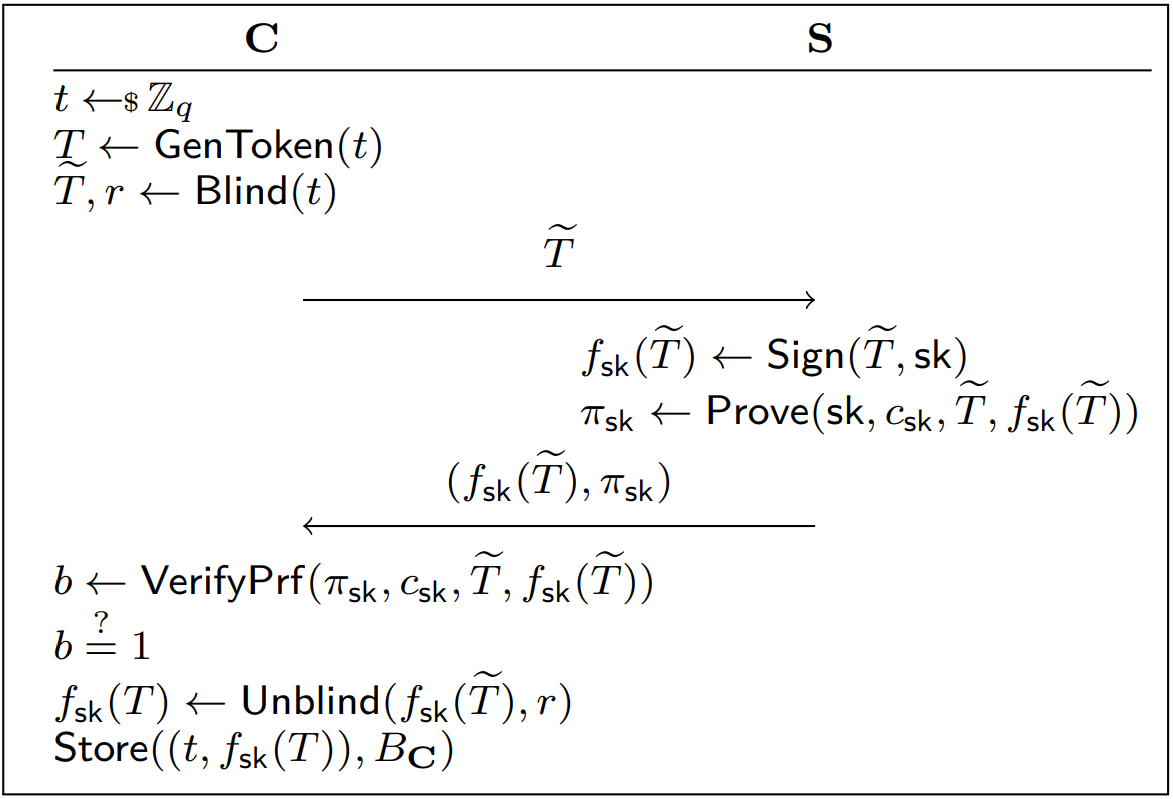
\includegraphics[width=0.5\linewidth]{pp_signphase.png}
    \caption{Signierphase von Privacy Pass \cite{pp-davidson2018privacy}}
    \label{fig:pp-signingphase}
\end{figure}
Zuerst erstellt der Nutzer \textit{C} (Client) einen Tokenseed $t$ mit $t {\in}_R \mathbb{Z}_q $. Daraus generiert er Token $T$ bspw. mit einer Hashfunktion und blindet diesen mit $r$ wie in \ref{sec:blindSig} beschrieben, um $\widetilde{T}$ zu erhalten. Dieser geblindete Token wird nun an der Server \textit{S} gesendet, damit dieser in signieren kann. Beim Server angekommen beginnt dieser damit, den Token mit seinem privaten Schlüsselt $sk$ zu signieren. Anschließend erstellt er einen sogenannten Batch Discrete Log Equivalence Proof (BDLEQ), um dem Nutzer zu beweisen, dass er nicht für jeden Nutzer einen eigenen privaten Schlüssel verwendet um ihn über längere Zeit zu deanonymisieren. Der signierte Token und der BDLEQ werden wieder an den Nutzer gesendet, dieser prüft die Korrektheit des Beweises, unblindet den signierten Token und speichert ihn für spätere Verwendung. 

\paragraph{Einlösephase} Signierten Token einlösen\\
\begin{figure}[H]
    \centering
    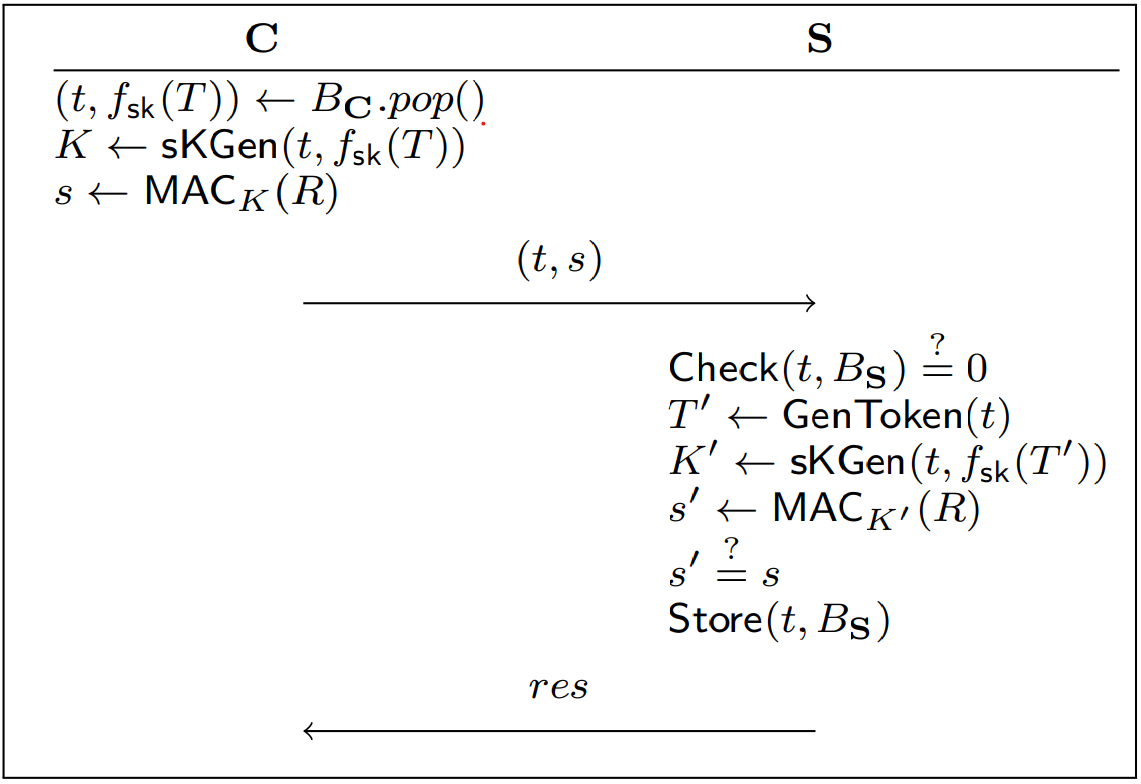
\includegraphics[width=0.5\linewidth]{pp-redemptionphase.png} 
    \caption{Einlösephase von Privacy Pass \cite{pp-davidson2018privacy}}
    \label{fig:pp-redemptoinphase}
\end{figure}
Der Nutzer beginnt damit einen gespeicherten signierten Token auszulesen und einen anfragenabhängigen Wert $R$ zu berechnen. Dieser könnte einfach die Domain der Anfrage sein. Er generiert einen shared key $K$ aus dem Tokenseed und dem signierten Token und verschlüsselt $R$ mit $K$ als key. Daraufhin sendet er das Tupel aus Tokenseed $t$ und $s\leftarrow MAC_{K}(R)$ mit shared key verschlüsseltem $R$ an den Server. Der Server prüft ob $t$ bereits für eine vorherige Anfrage verwendet wurde. Falls dies nicht der Fall ist, berechnet er auf Grundlage von $t$ alle Schritte des Nutzers und erhält so ein $s'$. Sollte $s'=s$ gelten, dann ist der Token valide, das CAPTCHA kann übersprungen werden und der Nutzer erhält Zugriff auf die angefragt Webressource.

Im Grund lässt Privacy Pass gut auf die Verwendung im Datentreuhändermodell anwenden. Unter den Annahmen, dass ein Datennutzender hier ein Nutzer ist, kann er Token bei dem Datentreuhänder erwerben, speichern und zu einem späteren Zeitpunkt wieder ausgeben. Da die Token blind signiert werden wird vermieden, dass der Datentreuhänder die in den unterschiedlichen Phasen verwendeten Token zueinander verlinken kann und Zusammenhänge zwischen einlösen und ausgeben ziehen kann. Der Datentreuhänder kann eine weitere überprüfende Instanz verwenden wie in \cite{pp-davidson2018privacy} beschrieben wird, um den Aufwand der Überprüfung auszulagern. \\
Einige Punkte sprechen jedoch gegen die direkte Verwendung von Privacy Pass. 
\begin{enumerate}
    \item Die Token haben keinen Wert. Bei Bezahlungsmittel ist es essentiell einen bestimmten Preis bezahlen zu können. Dafür wären entweder mehrere unterschiedliche Token von Nöten oder Token welche einen monetäre Wert gespeichet haben. Ansonsten kann nur in Vielfachen von dem einen Token gezahlt werden was dazu führt, dass es keine präzise Preisvergabe gibt oder bei jeder Transaktion eine große Menge an Token validiert werden müssen.
    \item Ein Nutzer interagiert sowohl zum Einlösen als auch zum Ausgeben nur mit dem Server und nicht mit einem Verkäufer dem er seine Token im Tausch anbietet. Es existiert hier also kein 3. Akteur wie bei GNU Taler \ref{subsec:gnu} der erhaltete Token einlöst.
    \item Die Token können ähnlich wie bei GNU Taler \ref{subsec:gnu} nicht direkt an den Verkäufer weitergegeben werden, da dadurch eine direkte Verbindung zwischen Datennutzenden und Datengebenden entsteht, welche schützenswerte Informationen an den Datennutzenden preisgibt.
\end{enumerate}

\section{Privacy-Preserving Reputation Management}
\label{subsec:rep}
In ihrem Paper beschreiben R Petrlic et al. ein Reputationssystem, um Nutzern den Dienst eines Dienstleisters anonym bewerten zu lassen und so anderen Nutzern eine Einschätzung über die Qualität der Dienstleistung zu geben \cite{petrlic2014privacy}. Es werden 3 Rollen charakterisiert. Ein Reputation Provider $RP$, der sich um das Verwalten der verschiedenen Reputationswerte kümmert. Eine Menge an Service Providern $SP$, welche einen Dienst anbieten, der durch Nutzer bewertet werden soll. Und zuletzt eine Menge an Nutzern $U$, die die Dienstleistung der Service Provider bewerten, wobei keiner der Nutzer gleichzeitig ein Service Provider $SP$ sein kann, $U \cap SP = \varnothing$. 

Der im Paper beschriebene Ablauf des Bewertens, eines $sp \in SP$ durch einen Nutzer $u \in U$, umfasst grob die Erstellung eines Schemas für einen Bewertungsvektors durch $sp$, welcher von $u$ später verwendet wird, um den $sp$ zu bewerten. Nach dem $sp$ dieser Vektor mit dem $RP$ kommuniziert wurde, kann $u$ eine Dienstleistung von $sp$ in Anspruch nehmen. Dieser antwortet, zusätzlich zur Erbringung der Dienstleistung, mit einer Beschreibung des Bewertungsvektors, einem Schlüsselpaar und einem Token. Dank der Beschreibung kann der Nutzer selbst einen Bewertungsvektor erstellen, in welchen er seine Bewertung der Dienstleistung einbaut. Im Anschluss wird dieser mit dem Schlüsselpaar verschlüsselt, signiert und zusammen mit dem signierten Token, an den $RP$ gesendet. Der Token dient hier zur Erkennung von doppelten Bewertungen. 

Die Berechnung der Reputation ist in Zeitslots eingeteilt, damit ein $sp$ nicht in der Lage ist einen alten Reputationswert anzugeben. Wenn nun ein Nutzer $u$ den Reputationswert eines $sp$'s einsehen möchte und der Wert für den gewünschten Zeitraum noch nicht bestimmt wurde, so muss dieser zwischen $RP$ und $sp$ berechnet werden. Hierfür bestimmt $RP$ die Summe aller verschlüsselten Bewertungsvektoren für den Zeitraum und sendet diese, zusammen mit weiteren Prüfwerten an $sp$. Dieser kann die übermittelten Werte prüfen und auf eine Blacklist hinzufügen, um Replay Attacken von $RP$ auszuschließen. Wenn die Überprüfung gelingt, signiert $sp$ die Summe der Vektoren zusammen mit einer ID und verifiziert somit den neuen Reputationswert an $RP$. 

Bei einer Anfrage des Reputationswertes von $sp$ durch $u$, schickt der $sp$ eine Reihe an Werte zu $u$. Diese erlauben es $u$, den Bewertungsvektor zu interpretieren und zu prüfen, dass der übermittelte Werte sowohl aktuell ist, als auch nicht beeinflusst wurde. 
Das Konzept von Petrlic et al. bietet unter anderem Schutz vor: 
\begin{enumerate}
    \item \textbf{Whitewashing}, bei welchem sich ein $sp$ mit schlechter Reputation als neuer $sp$ ausgeben kann, um somit den Wert zurücksetzen kann.
    \item \textbf{Transaction-independent Ratings}, bei welchen ein Nutzer die Dienstleistung bewerten kann, obwohl er besagt Dienstleistung nicht in Anspruch genommen hat.
    \item \textbf{Sybil Attacks}. Ein Nutzer bewertet eine Dienstleistung unter mehreren Identitäten und täuscht so seine Meinung als Gruppenmeinung vor.
    \item \textbf{Delta Analysis}. Eine teilweise Deanonymisierung des Nutzers durch vergleichen von gesammelten Bewertungen in unterschiedlichen Zeitabständen.
\end{enumerate} 
In der vorliegenden Situation kann das Konzept zu großen Teilen verwendet werden. Die Rollen können unter anderen Namen genauso verwendet werden. In diesem Fall wird der Service Provider zum Datengebenden, der Nutzer wird zum Datennutzenden und die zu bewertende Dienstleistung wird zu den übermittelten Daten. Allerdings ist das Konzept darauf ausgelegt, dass zu Beginn eine Kommunikation zwischen dem Datengebenden und Datennutzenden besteht, so dass der Reputationswert direkt vom Datennutzenden abgefragt wird. An dieser Stelle muss es also etwas abgewandelt werden, da zu Beginn keine direkte Kommunikation zwischen einem Datennutzender und einem Datengebenden besteht. Erst nachdem der Treuhänder dem Datennutzenden eine List an Datengebenden mitgeteilt hat, kann eine direkte Kommunikation entstehen. Stattdessen soll der Austausch des Reputationswertes  direkt über den Treuhänder geschehen.

\section{Blinde Signaturen}
\label{sec:blindSig}
Das von David Chaum im Jahre 1983 veröffentlichtes Paper ``Blind signatures for untraceable payments`` beschreibt den theoretischen Ansatz, dass ein Nutzer eine verifizierbare Signatur für eine Nachricht erhält, ohne dass der Unterzeichner den Inhalt der Nachricht kennt. \cite{chaum1983blind}. Ein Beispiel hierfür wäre ein Zahlungsdienstleister, der eine neuen Coin in dem Umlauf bringen möchte. Dafür sendet er seinen Reputationswert und den unkenntlich gemachten Coin an eine Zentrale Institution. Wenn diese den Reputationswert als hoch genug ansieht und somit den Zahlungsdienstleister als vertrauenswürdig erkennt, so kann sie den Coin blind signieren und an den Dienstleister zurückschicken. Wenn nun ein späterer Inhaber des Coins, prüfen möchte, ob sein Coin von einem vertrauenswürdigen Dienstleister erstellt wurde, so kann er die blinde Signatur mit dem öffentlichen Schlüssel der Institution entschlüsseln. Das Ergebnis dieser Berechnung zeigt, dass die Institution den Coin tatsächlich signiert hat und sie dem Coinaussteller vertraut. Der hierbei essentielle Punkt ist, dass diese Institution nicht weiß, was sie unterschreibt. Somit kann die Institution die Beziehung des Dienstleisters und des Coininhabers nicht nachverfolgen. 

Die für das Verfahren nötigen Rechenschritte sind im Folgenden beschrieben. Angenommen der Unterzeichnende verfügt über eine private Signierfunktion $s'$ und eine öffentliche Funktion $s$, sodass $s(s'(x)) = x$. Der Nutzer verfügt über die privaten Funktionen $c$ und dessen invers $c'$, sodass $c'(s'(c(x))) = s'(x)$. 
\begin{enumerate}
    \item Der Nutzer beginnt nun damit, sich ein $x$ auszusuchen. Dieses wird durch zufällige Redundanz vor Kollisionen geschützt und mit $c(x)$ unkenntlich gemacht.
    \item Anschließend erhält der Unterzeichnende $c(x)$, berechnet $s'(c(x))$ und schickt den entsprechenden Wert an den Nutzer zurück.
    \item Wenn der Nutzer nun $c'(s'(c(x))) = s'(x)$ berechnet, so erhält er den signierten Ursprungswert $x$ ohne, dass der Unterzeichnende $x$ je kannte.
\end{enumerate}
Daraufhin kann jede weitere Person die Unterschrift überprüfen, indem diese die öffentliche Funktion $s$ verwenden um $s(s'(x))$ zu berechnen und das Ergebnis mit $x$ abgleichen. 

Blinde Signaturen sind bei dem Ansatz von privatsphäreschützenden Zahlungs- und Reputationssystemen einer der Kernbausteine der verwendet wird, um einen vertrauenswürdigen Austausch zwischen den Parteien zu ermöglichen. Sie liefern die Grundlage der Kommunikation+0

\section{Partiell Blinde Signaturen}
\label{sec:partBlindSig}
Partiell blinde Signaturen ähneln sich vom Effekt stark zu blinden Signaturen von Chaum aus \ref{sec:blindSig}. Der jedoch entscheidende Unterschied ist, dass es bei partiell blinden Signaturen einen Infowert gibt der sowohl Nutzer als auch Signierende bekannt ist. Dieser kann genutzt werden, damit der Signierende möglicherweise Prüfung ausführen kann und zu entscheiden ob er die Nachricht wirklich signieren möchte. Diese Eigenschaft wird im späteren Verlauf bspw. dazu verwendet einen Coin partiell blind zu signieren. Hierbei ist es essentiell, dass der Signierende den monetäre Wert des Coins prüfen kann, da ein Nutzer sonst freie Kontrolle über den Wert seines eigenen Coins hat. Mit partiell blinden Signaturen, kann genau dies gewährleistet werden. Dabei ist die monetäre Wert des Coins die Info und der kryptographische Wert des Coins die Nachricht. Nun kann der Signierende prüfen, dass der monetäre Wert der vereinbarte Wert ist und kann den kryptographischen Wert des Coins blind signieren. Der springende Punkte ist der Zusammenhang zwischen Info und Nachricht, da sonst der monetäre Wert des Coins nach dem Signieren durch den Nutzer verändert werden könnte. Um dies zu verhindern, verwendet das Verfahren den Hash der Info als Teil der Signatur, so dass diese nur gültig ist, solange die Info unverändert bleibt.

\subsection{Funktionweise}

\begin{figure}[H]
    \label{fig:partBlindSig}
    \centering
    \includegraphics*[width=1\textwidth]{partBlindSig.png}
    \caption{Ablauf einer partiell blinden Signatur \cite{abe2000provably}}
\end{figure}

Die Durchführung einer partiell blinden Signatur besteht aus 4 Schritten. Diese 4 Schritte sind notwendig, um die Abhängigkeit von dem msg und info herzustellen. Es wird davon ausgegangen, dass vor dem ersten Schritt beide Parteien über den Infowert verfügen. Der Signierende bildet zuerst den Hashwert der info signiert diesen und schickt ihn an den Nutzer. Dieser bildet den gleichen Hashwert der info und verwendet die erhaltenen Werte zusammen mit einer Reihe an Zufallszahlen, um $\alpha$ und $\beta$ zu berechnen. $\epsilon$ ist der darauf folgende Hash von $\alpha,\beta,z$ und $msg$. Hier fließt die bereits signierte info über $\alpha$ und $\beta$ mit ein. Kurz darauf empfängt der Signierende $e$, welches nun sowohl info als auch msg beinhaltet. Dieses $e$ kann er nun verwenden, um info und msg zu signieren und die aus den Berechnungen resultierende Werte an den Nutzer zu senden. Der Nutzer kann dadurch $\rho,\omega,\sigma ,\delta$ zu bestimmen und zu speichern. Möchte der Nutzer zu einem beliebigen Zeitpunkt die Signatur auf ihre Gültigkeit prüfen, so kann er $\omega + \delta$ mit  $H (g^\rho y^\omega || g^\sigma z^\delta || z || msg)$ vergleichen. Wenn die Werte übereinstimmen, ist die Signatur valide.

Durch den Verwendung von info als Teil der Signatur ist gewährleistet, dass die Signatur nur bei einer unveränderten info und msg valide bleibt. Denn sollte sich die info oder msg ändern, dann würde die Rechnung zum Überprüfen einen anderen Hash erzeugen, welcher nicht mehr mit $\omega+\delta$ übereinstimmt. Insgesamt ist das partiell blinde Signaturen Schema etwas umständlicher als Chaums blinde Signaturen. Dennoch bietet es die Möglichkeit einen öffentlichen Wert zu kommunizieren und dessen nachträgliche Änderung zu verhindern.


\section{Elliptische Kurven Kryptographie}
\label{sec:ecc}
Die Kryptographie über elliptische Kurven (ECC - elliptic curve cryptography) ist ein Zweig der Kryptographie welcher bereits seit 1985 besteht \cite{ecc-miller1985use} und trotz dessen nur wenig Aufmerksamkeit genießt . Hierbei geht es um das Ver- und Entschlüsseln von Nachrichten anhand von Punkten auf einem elliptischer Graph, was verglichen mit der weit verbreiteten Faktorisierungskryptographie große Performanzsteigerung liefert.

\subsection{Trapdoor functions}
Das asymmetrische RSA Verschlüsselungsverfahren ist heute weltbekannt und wird in über 90\% der Onlinekommunikation verwendet \cite{ecc-rsa_amount}. Dessen Sicherheit basiert genauso wie die von ECC auf sog.  \textit{Trapdoor functions}. Ein Trapdoor function ist ein mathematisches Problem, welches in eine Richtung leicht zu berechnen ist, jedoch das Inverse enorm schwer. Im Falle von RSA ist die Trapdoor function das Faktorisierungsproblem. Es ist leicht 2 sehr große Zahlen miteinander zu multiplizieren. Allerdings ist es enorm schwer bei einem gegebenen Produkt dessen Faktoren zu bestimmen, insbesondere wenn die Faktoren jeweils Primzahlen sind. Dies ist der Grund weshalb RSA sicher ist und zuverlässig die Kommunikation schützt. Bei ECC ist die Trapdoor function, die die Sicherheit der Verschlüsselung ausmacht, eine andere. Jedoch kann anhand dieser, ein public und private key generiert werden wie es für asymmetrische Kryptographie nötig ist.
\subsection{Funktionsweise}
Um die Trapdoor function hinter ECC zu verstehen müssen wir uns zuerst elliptische Kurven anschauen. Die algebraische Struktur von Elliptische Kurven ist eine Gruppe, welche aus einer Menge von Punkten $M$ und einer binären Operationen $\circ$ auf 2 Punkten der Menge besteht. Die Definition einer Gruppe fordert, dass die Element die Eigenschaften der Assoziativität, Identität, Existenz eines inversen Elements und je nach Quelle auch Abgeschlossenheit erfüllen. \cite{ecc-aradi2016einfuhrung}\cite{ecc-bogopolskij2008introduction} Zudem müssen die Koordinaten aller Punkte $(x,y) \in M$ die in der Menge liegen aus dem endlichen Feld stammen, sowie die Gleichung:

\begin{equation}
    \label{ecc-equation}
    y^2 = x^3+ax+b
\end{equation} erfüllen. Zusammen bildet die Menge an Punkten $M$ einen Graph der je nach Wahl der Parameter $a,b$ einer Form aus Abbildung \ref{fig:ecc_1} ähnelt. Aufgrund der Gleichung \ref{ecc-equation} entsteht der Zusammenhang, dass ein Gerade durch 2 zufällig gewählte Punkte $P,Q \in M$,  den Graph immer an genau einer dritten Stelle schneidet. Zusätzlich ist der Graph an der X-Achse durch das $y^2$ gespiegelt. Mit diesen Eigenschaften kann nun die Operation $\circ$ definiert werden.\\
Diese arbeitet wie folgt: Bei Eingabe von $A,B \in M$ finde den invertierten dritten Schnittpunkt mit dem Graph. Dieser sei hier mit $C$ beschrieben. Ein Ausführung von $A \circ B = C$ ist in Abbildung \ref{fig:ecc_2} verdeutlicht.

\begin{figure}
    \centering
    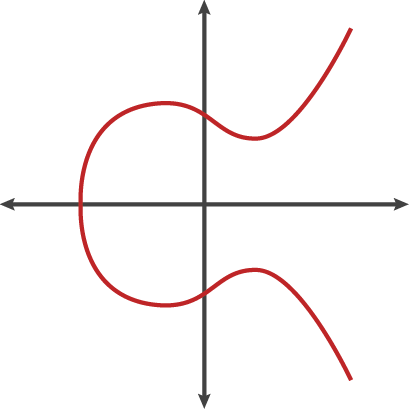
\includegraphics[width=0.4\textwidth]{ecc_1.png}
    \caption{Mögliche Form einer elliptischen Kurve \cite{ecc-cloud2013elliptic}}
    \label{fig:ecc_1}
\end{figure}
\begin{figure}
    \centering
    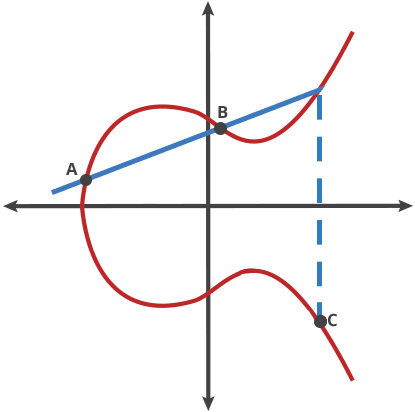
\includegraphics[width=0.4\textwidth]{ecc_2.png}
    \caption{Operation $\circ$ auf Punkten $A,B \in M$ \cite{ecc-cloud2013elliptic}}
    \label{fig:ecc_2}
\end{figure}
\begin{figure}
    \centering
    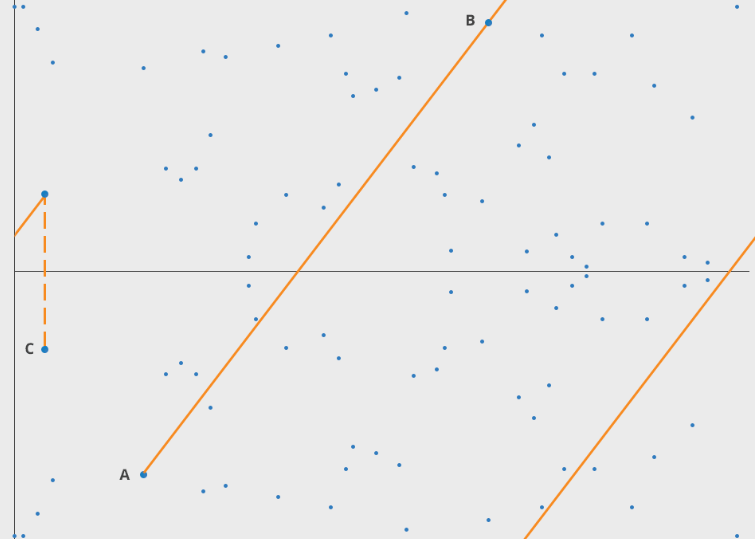
\includegraphics[width=0.4\textwidth]{ecc_3.png}
    \caption{Graph nach Anwendung von $\mathbb{Z}_p$ \cite{ecc-cloud2013elliptic}}
    \label{fig:ecc_3}
\end{figure}

Die Operation $\circ$ kann beliebig oft hintereinander mit dem jeweils neu entstehenden Punkt ausgeführt werden. Genau hier liegt die Trapdoor function von ECC. Mit Kenntnissen über der Startpunkt $A$ und die Anzahl der Ausführungen $n$, ist es einfach den Endpunkt $E$ zu berechnen. Wenn allerdings nur der Endpunkt $E$ und Startpunkt $A$ gegeben sind, ist es sehr rechenaufwändig die Anzahl an Ausführungen zu bestimmen.

\subsection{Anwendung in der Kryptographie}
Allgemein ist zu beachten, dass elliptische Kurven die für ein kryptographischen Verwendung in Frage kommen, eine andere Form haben, als die eben aufgeführt Abbildungen (\ref{fig:ecc_1},\ref{fig:ecc_2}). Entscheidend ist hierfür die Wahl des endlichen Feldes. In der Kryptographie wird hier meist $\mathbb{Z}_p$ verwendet. Diese Wahl bringt 2 Eigenschaften mit sich:
\begin{enumerate}
    \item Das $p$ in $\mathbb{Z}_p$ besagt, dass alle Werte $x \in \mathbb{Z}_p$, $0 \leq x \leq p-1$ erfüllen müssen. Durch die Wahl dieses Wertebereichs, können die X und Y-Achse nie den Wert $p$ überschreiten sondern beginnt anstatt wieder bei 0.
    \item Die zweite Eigenschaft ist die ausschließliche Betrachtung ganzer Zahlen als X und Y-Koordinate. Hierdurch wird aus dem Graphen eine Menge an zufällig aussehend gewählten Punkten. Der Graph für die kryptographische Verwendung einer elliptische Kurve ist ein Abbildung \ref{fig:ecc_3} visualisiert.
\end{enumerate}
Nun muss ein passendes $p$ sowie $a,b$ bestimmt werden, um die genaue Menge an Punkten zu spezifizieren. Hierfür gibt es bereits ein große Auswahl und Werten in der Literatur \cite{ecc-lochter2010elliptic}\cite{ecc-merkle2013elliptic}. Eine der prominentesten ist die ``Curve25519`` von Daniel J.Bernstein \cite{ecc-bernstein2006curve25519}. Sie hat den Werte $p=2^{255}-19$ (daher der Name) und die elliptische Funktion  $y^2=x^3+486662x^2+x$.


\subsection{Vor und Nachteile}
Allgemein betrachtet ist die Tatsache, dass ECC eine schneller Berechnungszeit liefert als RSA, nicht von der Hand zu weisen \cite{ecc-cloud2013elliptic}. Da die Laufzeiten von Verschlüsselung und Entschlüsselung durch RSA und ECC asymptotisch nicht gleich verhalten ist es schwer eine endgültige Antwort zu nennen. Allerdings schlägt ECC RSA bei der Gesamtzeit für Ver- und Entschlüsselung je nach Nachrichtengröße um einen Faktor von \textasciitilde $3-20$ \cite{ecc-mahto2018performance}\cite{ecc-bao2022research}. Zudem ist eignet sich ECC vorallem als Ver- und Entschlüsselungsmethode auf rechenschwachen Geräte wie Mobiltelefonen aufgrund von kleineren Schlüsselgrößen\footnote{Um eine security bit level von 256bits mit RSA zu erreichen, ist eine Schlüssellänge von 15360bits nötig während es bei ECC lediglich 512bits sind.\cite{ecc-mahto2018performance}}. So können Rechenaufwand, Energieverbrauch und RAM-Auslastung gesenkt werden \cite{ecc-gupta2011ecc}.

Allerdings wurde 2007 bekannt, dass der Pseudo Random Number Generator (PRNG) Dual\_EC\_DRBG eine potentielle Backdoor hatte, die es Nutzern mit Informationen über einen Wert die Zufälligkeit problemlos knacken lies \cite{ecc-green2013backdoor}. Dual\_EC\_DRBG wurde 2005-2006 zusammen von NIST (National Institute of Standarts and Technology) und der NSA veröffentlicht und basiert die Auswahl der zurück gegebenen pseudozufälligen Zahlen auf Berechnung über elliptischen Kurven. Dieser Vorfall schwächt bis heute das generelle Vertrauen in ECC.

\cite{ecc-cloud2013elliptic}

\section{Abschluss}
%pro und  contra von allen

%==================================================================================================



\chapter{Entwurf der Systeme}
%ziel, welche betrugserkennung, geld als Anreiz, soll hauptsächlich verkäufer schützen, eigene coins, exchange als neuer akteur, ecc


%erstellt und signiert coins, grober ablauf, auf welchem rl basiert, präziser ablauf in der Schrittbeschreibung

%bezahlung, grober ablauf, auf welchem rl basiert, präziser ablauf in der Schrittbeschreibung

%reputation, grober ablauf, auf welchem rl basiert, präziser ablauf in der Schrittbeschreibung

\section{Ziel}
Um einen privatsphäreschützenden Anreiz für die Benutzung eines Datentreuhänders zu schaffen, wird im folgenden ein Bezahlsystem vorgestellt. Dieses Bezahlsystem erlaubt es Datengebenden für ihre Daten im gegenzug einen finanziellen Ausgleich zu verlangen, ohne dabei persönliche Informationen preisgeben zu müssen. Weder der Datennutzende noch der Datentreuhänder kann bei einer regulären Transaktion bestimmen, welcher Datengebende ein Bezahlung erhält. Der hierfür vorgesehen Ablauf sieht vor, dass ein Datengebender zuerst seine Daten an den Datennutzenden überträgt und ihm etwas Zeit zur Verwertung der Daten lässt. Ein Datennutzender erhält maxmimal 3 Tage Zeit, um den Zahlvorgang abzuschließen. Tut er dies nicht innerhalb der 3 Tagen, so kann der Datentreuhänder ihn von der weiteren Verwendung der Plattform ausschließen. 

Damit der Datengebende seine Anonymität nicht ausnutzen kann, gibt es 2 Mechanismen zur Betrugserkennung. Der erste ist eine Offenlegung der Kommunikation im Streitfall. Sollte sich eine der beiden Parteien betrogen fühlen, so kann sie vom Datentreuhänder eine Schlichtung verlangen. Dafür werden die für die Kommunikation verwendeten Einmalschlüssel dem Datentreuhänder mitgeteilt, sodass dieser alle Schritte nachvollziehen kann und entscheiden kann ob ein Betrug vorliegt oder nicht. 

Der zweite Mechanismus ist eine Reputationsvergabe. Wenn ein Datengebender besonders qualitativ gute Daten liefert, wird er durch den Datennutzenden mehr bezahlt, was sich in der Reputation widerspiegelt. Wenn er hingegen besonders schlechte Daten liefert, so kann ein Datennutzender sich weigern ihn zu bezahlen, was die Reputation runter zieht. So kann bei jeder Nachfrage nach Daten von einem Datennutzenden ein Reputationsschwellwert festgelegt werden, um Datengebende mit zu schlechter Reputation vor dem einreichen ihrer Daten abzuhalten. 

\section{Geld als Anreiz}
Da im Datentreuhandmodell ein Datennutzender meist durch ein Unternehmen oder eine Forschungseinrichtung repräsentiert wird, ist es verstellbar, dass der Datennutzende selbst eine Dienstleistung anbieten oder in Aussicht stellen kann. Hier wurde aber Geld als Anreiz gewählt, da die Verwendung solcher Dienstleistungen als Anreiz einige Nachteile mit sich ziehen kann.

\begin{enumerate}
    \item \textbf{Begehrtheit} Kein Handelsgut oder Dienstleistung ist so universelles begehrt wie Geld. Zwar ist es möglich das ein Business welches hier als Datennutzender auftritt, für die Preisgabe der Daten eine Dienstleistung anbietet. Bspw. können Social Media Plattformen wie X konstenlose zeitlichbedingte Premiumabonnenments oder vergleichbar Angebote in Aussicht stellen. Jedoch sind ist das Interesse an solchen Angeboten subjektiv, was sie als mögliche Anreize zwar denkbar aber eher suboptimal macht.
    \item \textbf{Hoher Aufwand} Wenn der Anreiz durch den Datennutzende gestellt wird, wird dieser in jedem einzelnen Fall unterschiedlich sein. Aus der Kommunukationsstruktur folgt das alle unterschiedlichen Kompensationen auf irgendeinem Weg über der Datentreuhänder laufen müssen. Daraus ergibt sich einen enormer zusätzlicher Aufwand an Entwicklung und Implementation für jeden Datennutzenden.
    \item \textbf{Verfügbarkeit} Manche Datennutzende wie bspw. Forschungsinstitutionen haben keine Dienstleistungen oder Produkte die sie Datengebenden anbieten können. Sie sind ausschließlich an der Forschung interessiert und können den Datengebenden nichts bieten was sie zum preisgeben ihrer Daten veranlassen würde.
    \item \textbf{Wahrung der Anonymität} Viele C2B Treuhänder legen Wert auf die Anonymität oder Pseudonymität der Datengeber. Diese kann jedoch dadurch, dass eine Datennutzender die versprochene Dienstleistung kontrolliert verloren gehen. Es ist bspw. denkbar dass ein Datennutzender eine vielversprechenden Anreiz verspricht, diesen aber hinter einer Registrierung und Angaben von persönlichen Daten verbirgt, so dass die durch den Treuhänder etablierte anonymität umgangen wird.
    \item \textbf{Einhalt der Leistung} Der Datentreuhänder kann bei der Auslagerung von Anreizen an den Datennutzenden nicht zuverlässig kontrollieren, dass der Datennutzende die versprochene Dienstleistung wirklich einhält.
\end{enumerate}
Durch eine die Verwendung von Geld als Anreiz werden diese Punkte umgangen. Das Interesse der Datengebenden ist nun ausschließlich abhängig von dem Ruf und dem persönlichen Interesse an einem Datengebenden und nicht von dessen Anreizangebot. Die in Anspruchnahme des versprochenen Anreizes ist für jeden Datennutzenden gleich Implementiert und hängt maximal von der Wahl anderer Parameter ab. Es kann davon ausgegangen werden dass alle Datennutzenden über Geld verfügen und dieses als Kompensation verwenden können. Aufgrund der (trivialität?) des Wertes von Geld sind bereits viele Wegen bekannt wie diesen Wert anonym oder pseudony an andere überträgt. Der Datentreuhänder hat die volle Kontrolle, dass ein zu zahlender Geldbetrag vom Datennutzenden abgegeben wird und auch bei Datengebenden ankommt.
 

\section{Generelles}
Im gegensatz zu GNU Taler soll das Bezahlsystem hauptsächlich den Datengebenden und dessen Informationen schützen. Die privatsphäre des Datennutzenden ist von geringerer Bedeutung, da im Datentreuhändermodell der Datennutzende meist durch ein Unternehmen oder eine Forschungseinrichtung dargestellt wird. Hinzu kommt dass durch die Struktur eines Datentreuhänders, der Datennutzende dazu gezwungen ist eine Menge an Informationen anzugeben, um vom Datentreuhänder zugelassen zu werden. Der Datengebende hingegen ist eine einzelne Privatperson die ihre gesammelten Daten bewusst an Unternehmen oder Forschungseinrichtungen verkaufen möchte. Der Schutz der Privatperson ist hier also von größerem Interesse. 

Unter diesen Umständen ist eine herkömmliche Überweisung per Bank deutlich zu unsicher. Sie benötigt Information wie die IBAN des belasteten Kontos und die IBAN des empfangenden Kontos, um zu wissen von wo nach wo eine Geldsumme fließen soll. Dadurch werden bereits zu viele Informationen über den Datengebenden bekannt, da der Datennutzende nun genau bestimmen kann von wem die erworbenen Daten stammen und ob er bereits vorher schon von demselben Datengebenden Daten gekauft hat. Zusätzlich kann die Bank nachvollziehen, dass eine Privatperson sich als Datengebender angemeldet hat und wem sie ihre Daten bereits verkauft hat.
Um dieses Problem zu lösen wird hier eine der gängigsten anonymen Onlinezahlmethoden verwendet: Kryptowährungen. Die Abschnitte \ref{subsec:gnu}, \ref{sec:bitcoin}, \ref{sec:ethereum}, \ref{sec:privacy-pass} führen bereits wenige davon auf und beschreiben warum sie nicht im Datentreuhändermodell verwendbar sind. Aufgrund dessen wird hier eine neuer Coin eingeführt. Jedoch ist dieser weder Blockchain basiert, noch für Spekulationszwecke geeignet. Ein Coin kann - so wie bei den meisten Kryptowährungen - ausschließlich bei einem Exchange gegen Geld getauscht werden. Bei dem initialen tauschen mehrerer Coins ist der monetäre Wert in Euro fest im Coin gespeichert und kann nicht verändert werden. 

An dieser Stelle ist anzumerken, dass keine Regulierungen oder Identifizierung zum erwerben eines Coins benötigt werden. Jedoch sind Datennutzende die einzigen die Coins sicher ausgegeben können, da das Bezahlsystem nur dazu verwendet werden kann, Coins von Datennutzenden zu Datengebenden zu übertragen. Datengebende können zwar selbst auch Coins erwerben, allerdings ist der Handel nicht über dass hier eingeführt Bezahlsystem möglich. Daher bleibt nur der reguläre Tausch, welcher außerhalb des Systems stattfindet und keine Betrugserkennung besitzt. Unter der Berücksichtung dass das einzige was dem Coin einen festen Wert sicher stellt, die Signatur des Exchanges ist, kann leicht ein nicht verifizierter Coin erstellt werden und im unsicheren Tausch angeboten werden. Der andere Tauschpartner hat keine Möglichkeit den Coin vor Abwicklung des Tauschs auf seine Echtheit zu prüfen, was ein riesen Potentiall für Betrug zulässt. Aufgrund dessen ist anzunehmen, dass nur Datennutzende Coin erwerben werden, da der Tausch unter Datengebenden deutlich zu unsicher ist.

Nachdem ein Datennutzender einen Coin erworben hat, kann er diesem lokal speichern bis er ihn ausgeben möchte. Sobald sich ein Datengebender seine Daten mitteilt, hat der Datennutzende 3 Tage Zeit die Daten auszuwerten. Während dieser 3 Tage kann er maximal von 10 Datengebenden Daten empfangen. Dies ist ein Schutzmechanismus der einen bösartigen Datennutzenden daran hindert unbegrenzt Daten zu sammeln ohne für diese zu bezahlen. Es ist denkbar den Wert bei Datennutzenden welche bereits lange ohne Betrug agieren zu erhöhen um eine bessere Parallelisierung der Verarbeitung zuzulassen. Wenn ein Datennutzender nach Ablauf der 3 Tage noch keine Transaktion zu dem Datengebenden abgeschlossen hat und dieser bei dem Datentreuhänder eine Betrugsanklage gegen den Datennutzenden vorlegt, so kann der Datentreuhänder sich dazu entschließen den Datennutzenden entweder zeitlich bedingt oder dauerhauft von der weiteren Verwendung der Plattform auszuschließen. Ein gutwilliger Datennutzender kann nach der Auswertung der Daten eine passende Summe an Coins aus seinem lokal speicher auslesen und an den Datengebenden sendet. Sobald dieser die Coins empfängt, prüft er die Signatur der Coins. Wenn diese mit der des Exchanges übereinstimmt, leitet er sie an den Exchange weiter um sich den monetären Wert auf sein auf bspw.  seinem Konto gut schreiben zu lassen. Stimmt die Signatur nicht mit der des Exchanges überein, so kann der Datengebende auch hier wieder einen Betrug beim Datentreuhänder melden.

% ABSATZ ZU REPUTATIONSVERGABE

\section{Verschlüsselung}
Da in der Kommunikation indirekt Geld transferiert wird, ist es von höhster Priorität, die gesendeten Nachrichten vor dem Mithören oder Verändern durch unbefugte dritte zu schützen. Für diesen Schutz wird die in \ref{sec:ecc} erklärte elliptische Kurven Kryptographie verwendet. Mit der Verwendung des public keys des Empfängers wird sichergestellt, dass nur Personen mit Wissen über den zugehörigen private key die Nachricht lesen können. Gleichzeitig wird ein Hash der unverschlüsselten Nachricht gebildet und mit dem private key des Sender signiert. Auf diesem Weg kann der Empfänger die Nachricht entschlüsseln, selbst den Hash bilden und prüfen ob der signierte Hash mit dem selbst gebildeten übereinstimmt. Dadurch kann sowohl die Vertraulichkeit als auch die Integrität der Nachricht sichergestellt werden.

\section{Coin Generierungsphase}
Hier werden die Coins die im späteren Verlauf beider Systeme verwendet werden vom Datennutzenden erstellt und vom Datentreuhänder signiert. Die einzelnen Schritte sind in Abbildung \ref{fig:coin-generationphase} verdeutlich und werden im folgenden beschrieben.
\begin{figure}[H]
    \centering
    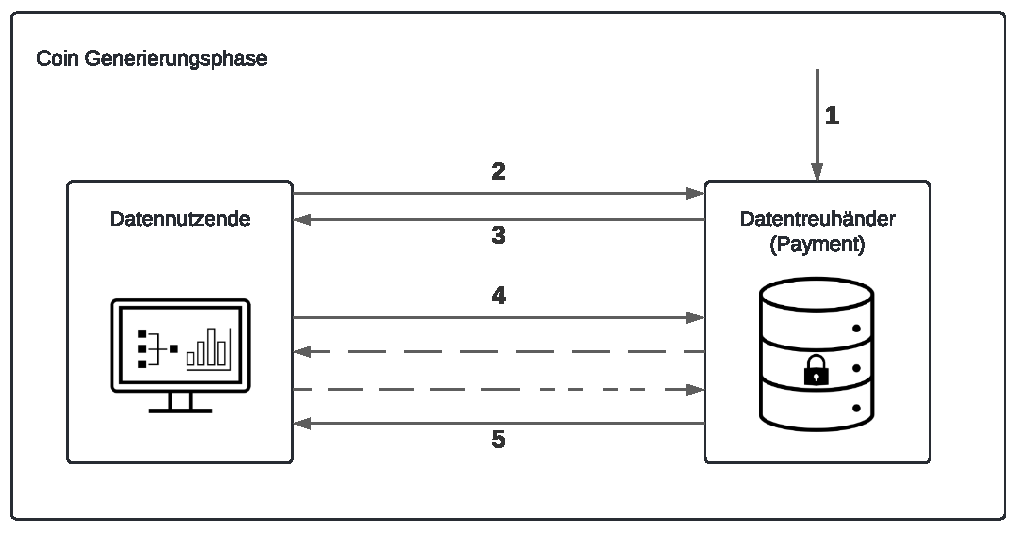
\includegraphics[width=0.9\linewidth]{CoinGenerationPhaseDiagramm.pdf}
    \caption{Coin Generierungsphase Ablauf}
    \label{fig:coin-generationphase}
\end{figure}

\paragraph{1. Zahlungseingang} $(apk \leftarrow AccountPublicKey, ES \leftarrow ErhalteneSumme)$\\
Der Exchange erhält über einen beliebigen Weg eine Summe und einen Konto public key. Die genaue Umsetzung des Zahlungseingang liegt bei dem Exchange. Er kann alles zwischen einer Banküberweisung mit der $apk$ als Verwendungszweck, bis hin zu einem Briefumschlag mit Bargeld und einem leserlich aufgeschriebenen $apk$ sein. Nach Eingang einer Zahlung erstellt der Exchange einen sogenannten CoinGenerationToken bestehend aus $(nonce, apk, ES, spent \leftarrow false)$, verschlüsselt ihn mit dem $apk$ und speichert diesen intern.

\paragraph{2. CoinGenerationToken abrufen} $(apk)$\\
Da der Exchange nur den $apk$ erhält, hat er keine Möglichkeit den CoinGenerationToken einem Datennutzenden zuzuweisen. Jetzt kann jeder beliebige Nutzer alle Einträge für einen $apk$ abfragen. Allerdings ist nur der Datennutzende in der Lage den CoinGenerationToken zu entschlüsseln, der den passenden secret key zum $apk$ hat. Dies ist im Idealfall nur der Datennutzende der die Transaktion getätigt hat.

\paragraph{3. CoinGenerationToken übertragen} $[(nonce, apk, ES)]$\\
Auf eine CoinGenerationToken Anfrage des Datennutzenden antwortet der Exchange mit allen noch nicht eingelösten Token für den $apk$. Nachdem der Datennutzende die Token erhalten hat, kann er diesen zuerst mit dem passenden secret key entschlüsseln. Im Anschluss kann er selbst Coins erstellen. Ein Coin besteht aus $(nonce, value)$. Bei der Erstellung sind 2 Sachen zu beachten. Zuerst muss der summierte Wert aller erstellten Coins gleichgroß sein wie die $ES$ des Tokens. Des weiteren gibt es eine Menge an möglichen Werten $PV$, sodass $\forall value\in  PV$ gilt. Dies ist vor allem wichtig, da $value$ beim Signieren und Einlösen des Coins für den Exchange sichtbar ist und dieser bei einer Wahl von selten vorkommenden $value$ ein Verbindung zwischen den Phasen herstellen kann.

\paragraph{4. Signierung Anfragen} $(nonce, apk, ES), [(value)]$

Eine Signieranfrage ist der Start eines Durchlaufs von partiell blinden Signaturen, bestehend aus einem CoinGenerationToken und einer Menge an $values$. Zuerst kann der Exchange prüfen ob der gesendete Token noch nicht eingelöst wurde. Anschließend summiert er alle $value$ auf und prüft ob die Summe gleich dem $ES$ des Tokens ist. Wenn beide Überprüfungen akzeptieren, kann der Exchange mit dem partiell blind signieren anfangen und bei seinem gespeichert Token $spent \leftarrow true$ setzen, um eine doppelte Einlösung zu verhindern.

\paragraph*{Gestrichelte Pfeile} $[(a,b)], [(e)]$\\
Die Pfeile zwischen 4. und 5. sind hier gestrichelt eingetragen, da sie notwendige Kommunikationsschritte von partiell blinden Signaturen abbilden. Sie sind essentiell für die Funktionsweise und wurden bereits in \ref{sec:partBlindSig} erklärt, weshalb sie hier nur zur Vollständigkeit aufgelistet werden.

\paragraph{5. Signieranfrage Antwort} $[(r,c,s,d)]$ \\
Vorrausgesetzt alle Überprüfungen aus Schritt 4 akzeptieren, so erhält der Datennutzende nun eine Menge an partiell blinden signierten Coins und kann diese für spätere Verwendung lokal speichern. Sollten die Überprüfungen nicht akzeptieren, so kann der Datennutzende entweder bei Schritt 4 mit anderen Coins oder bei Schritt 2 wieder ansetzen.\\\\

Auf diese Weise kann ein Datennutzender Geld bei einem Exchange einzahlen und eine dem Geldbetrag entsprechende Menge an Coins erhalten, ohne dass der Exchange die von ihm ausgehändigten Coins nachverfolgen kann. Gleichzeitig ist es für einen Datennutzende nicht möglich Coins zu erhalten für die er keinen monetären Gegenwert bereitgestellt hat.\\\\

Zusätzlich ist zu erwähnen, dass Exchanges finanziell motiviert sein können oder eine Gebühr verlangen möchten, um bspw. laufende Serverkosten zu decken. Sollte dies der Fall sein, kann vor dem Beginn der Coin Generationphase vom dem Exchange eine feste Gebühr vorgeschrieben werden. Wenn sich ein Datennutzender trotz der Gebühr dazu entscheidet diesen Exchange zu verwenden, so kann der Exchange nach dem Eingang einer Zahlung in Schritt 1, einen CoinGenerationToken erstellen, welcher die Gebühr bereits abzieht. Wenn also ein Datennutzender eine Transaktion von $100$\texteuro  bei Exchange mit $10\%$ Gebühr tätigt, so erstellt der Exchange einen CoinGenerationToken für den angegebenen $apk$ mit $ES \leftarrow 90$\texteuro. Dadurch kann eine Exchange seine finanziellen Interessen geltend machen. Auch wenn es nicht das Ziel eines Exchanges sein sollte wirtschaftlich zu handeln, lässt so immerhin verhindern, dass ein Exchange mit den Betriebskosten Minus macht.

\section{Bezahlvorgang}

\section{Reputationsvergabe}


%==================================================================================================


\chapter{Implementation}
Wird kurz gehalten. Implementierung beschreiben

\section{TRESOR Projekt}

%==================================================================================================

\chapter{Auswertung}
Evaluation ist wichtiger als guter Ansatz

Sicherheit gegen Angreifer Modelle:
    - Honest but curios DT
    - bösartige DN



Graphs and Stats to make:
ECC vs RSA
weighted shifting average vs linear reputation calculation
security bit level performance

\section{Setup / Implementation}

\section{Metrics}

%==================================================================================================


\chapter{Bewertung}

\section{Erfüllen der Anforderungen}

\section{Research question 1}

\section{Research question 2}

\section{(Discussion)}


%==================================================================================================


\chapter{Begrenzungen}


%==================================================================================================


\chapter{Zusammenfassung}


%==================================================================================================



\thispagestyle{empty}

\vspace*{\fill}
\pagestyle{empty}

{
    \normalsize
    \begin{center}
        \textbf{Eidesstattliche Erklärung}
    \end{center}
    Hiermit versichere ich an Eides statt, dass ich die vorliegende Arbeit im Bachelorstudiengang Software-System-Entwicklung
    selbstständig verfasst und keine anderen als die angegebenen Hilfsmittel –- insbesondere keine im Quellenverzeichnis nicht benannten Internet-Quellen –- benutzt habe. Alle Stellen, die wörtlich oder sinngemäß aus Veröffentlichungen entnommen wurden, sind als solche kenntlich gemacht. Ich versichere weiterhin, dass ich die Arbeit vorher nicht in einem anderen Prüfungsverfahren eingereicht habe.
    \vspace*{1cm}\\
    Hamburg, den \today
    \hspace*{\fill}\begin{tabular}{@{}l@{}}\hline
    \makebox[5cm]{Knut Hoffmeister}
    \end{tabular}
    \vspace*{3cm}
}
\vspace*{\fill}

\printbibliography

\end{document}